\chapter{Multi-Cell System Performance under Exponential Correlated Shadow Fading}\label{ch:4}
 \par In a multi-cell cellular network, connections between the Base Station (BS) and Mobile Stations (MSs) may be discrupted when the channel has low signal-to-interference-plus-noise ratio (SINR). Shadow fading is a large-scale fading, which can significantly affect signal strength and reduce SINR for a large area. \reminder{add a sentence why the shadow fading is always corrected, e.g., cuased by an obstacle} Correlated shadow fading will result in correlated long-lasting outage durations in a multi-cell system. \reminder{Corrected shadow fading cause outage in large area, then you can say in a mobile network, it will cause long lasting outage. You should really expand the following sentence. 1. Delay sensitive traffic will be affected by shadowing, 2. Diversity is a way to address, thus add more BSs} Increasing the BS density to make the network denser is a common way to increase SINR, reduce the number of long-lasting outage durations and provide better Quality of Service (QoS) support for delay sensitive applications. In Chapter \ref{ch:2} and Chapter \ref{ch:3}, we discussed mitigating shadow fading in a single-cell model. In this chapter, we focuses on the study of the performance of a multi-cell communication system under correlated shadow fading. We consider the downlink direction in a multi-cell communication system. The outage probability of grid model and random model are presented given correlated shadow fading and different BS densities. First, we compare the outage probability of the two different BS layout models with the same\reminder{what do you mean by same} correlated shadow fading. Simulation results indicate that the Grid model \reminder{Grid model->grid model, also change Random model->random model} has better performance than the Random model. Secondly, the outage probability with independent shadow fading or correlated shadow fading for the Random model is demonstrated. SINR is calculated under the assumption of the existing independent shadow fading and correlated shadow fading. Thirdly, we focus on the more realistic Random model, and present the distribution of outage durations given independent shadow fading or correlated shadow fading. Simulation results demonstrate that, outage durations with correlated shadow fading are longer than those with the independent shadow fading. At the end, we show that increasing the BS density can mitigate the effect of correlated shadow fading and improve the system performance by reducing the outage probability and shortening outage durations. 
 
 \section{Background}
 %\par In a cellular communication system, the connection between the BS and a MS may be dropped when the user enters a deeply shadowed area. Fading phenomena can substantially affect the performance of a wireless communication system. In general, fading can be divided into two categories: large-scale fading and small-scale fading. A signal transmitted from source to destination will experience both large-scale and small-scale fading. Small-scale fading is caused by multipath propagation. Large-scale fading, which is also known as shadow fading, is caused by obstacles (trees, buildings, etc.) in the propagation path. In most cases, shadow fading is assumed to be temporally and spatially independent \cite{rappaport1996wireless}.  Researchers have also shown that shadow fading is spatially correlated at different positions on the propagation path \cite{gudmundson1991correlation}, \cite{zhang2008novel}. In \cite{fabbri2009impact} and \cite{patwari2008effects}, the effects of correlated shadowing in connectivity is demonstrated, which indicates that reliable connectivity will be much more difficult to maintain than indicated by independent shadow fading models. The spatial correlation of shadow fading is important when studying the quality of service of a mobile system since it will result in long-lasting outage durations, which will deteriorate the performance of the applications running on the network. The focus of this chapter is to study channel variations and system performance due to correlated shadow fading in a multi-cell communication system and provide a solution to reduce the frequency and duration of dropped connections and improve system performance by increasing BS density.
 
 
 
 \par There have been a lot of studies on the outage probability of cellular communication systems \cite{abu1991outage, petrovic2013outage, emamian2014outage}. The author of \cite{vural2015effect} analyzed the outage probability and coverage area under \emph{i.i.d} shadow fading, which follows Log-normal distribution, Weibull distribution and Gamma distribution. In contrast, there is much less work on the outage probability and outage duration, given the correlated shadow fading. However, performance of a multi-cell system with correlated shadow fading remains to be an open problem. In \cite{lu2015long} and \cite{lu2015shining}, we discussed the outage probability and the outage duration distribution of a single-cell communication system under the exponentially correlated shadow fading and the distance-angle correlated shadow fading. For a single-cell model, exponentially correlated shadow fading can be modeled as a Markov chain model. Highly correlated shadow fading will result in long-lasting outage durations. In \cite{lu2015shining}, a single-cell model under the distance-angle correlated shadow fading is investigated. The correlated shadow fading leads to correlated outage events and long-lasting outage durations. To overcome these disadvantages, we propose a cooperative communication scheme to mitigate shadow fading by deploying relays at the cell edge. Chapter \ref{ch:2} and Chapter \ref{ch:3} are limited to the single-cell model. In this chapter, we are going to extend the study to review the impact of correlated shadow fading on a multi-cell model, and provide a solution to overcome the long-lasting outage durations.
 
 
 
 \par For the multi-cell system, a new general model for the user SINR was developed using stochastic geometry \cite{andrews2011tractable}. The cellular network was modeled by placing BSs at locations as a homogeneous Poisson Point Process (PPP). The author concluded that, under general fading, increasing the number of BS did not affect the coverage probability and/or the outage probability, as long as the MS was connecting to the nearest BS. Moreover, the paper did a comparison between the grid model and the PPP model, and concluded that the regular grid model provided the upper bound of the coverage probability while the PPP model provided the lower bound. The author also considered the effect of independent log-normal interference, and concluded that, higher log-normal interference increases coverage probability, which is counter-intuitive. However,the author did not consider the scenario with correlated log-normal shadow fading. 
 
 
 
 \par A comparative analysis of the random topology and the grid topology of a small cell network deployment was given in \cite{chen2012small}. In this paper, the spatial outage probability and the spatial average throughput, versus the number of access points of the two different network deployments were illustrated under independent shadow fading. Approximate the outage probability and the capacity for $\kappa-\mu$ shadow fading was discussed in \cite{kumar2015approximate}. $\kappa-\mu$ shadow fading includes one-side Gaussian, the Rayleigh, the Nakagami-m and the Rician. As we mentioned before, the empirical measurements didn't exhibit such complicated features of shadow fading. Therefore, those complex features are not the main focus when investigating system performance under correlated shadow fading.
 \reminder{You might want to change the following to: We analyzed, we investigated}
 \par The key contributions of this chapter are summarized as follows:
 \begin{itemize}
 \item Analyze the relationship between correlated shadow fading and correlated outage events under correlated outage fields.. 
 \item Investigate outage probability of both the Grid model and the Random model given correlated shadow fading.
 \item Illustrate how increasing the BS density helps mitigate the correlated shadow fading for the Random model in terms of reducing the outage probability (coverage probability) and the percentage of long-lasting outage durations.
 \item Analyze the relation between the tunable parameter (de-correlation distance) of the correlated shadow fading model and the outage probability.
 \item Compare the performance of the system with regard to different MS-BS connection strategies: MS connecting to the nearest BS versus MS connecting to the BS providing strongest signal.
 \end{itemize}
 The chapter is organized as follows: Section \ref{4:CorrShadowField} presents the correlated shadow fading model used in this chapter and the resultant correlated outage field. Section \ref{4:SystemModel} illustrates the system model with two different BS deployments and investigates the outage probability given the two deployments. Section \ref{4:OutageProb} gives a theoretical analysis of the outage probability given correlated shadow fading. Section \ref{4:SimuProb} presents the simulation setup and analyzes the simulation results from different BS densities. Section \ref{4:Conclusion} summarizes the chapter and proposes future work directions.
 
 \section{Correlated Shadow Fading}
 \label{4:CorrShadowField}
 As stated in Chapter \ref{ch:2}, empirical measurements show that correlation patterns varies between locations. Independent log-normal shadow fading model, while very useful for static MS performance analysis, does reflect the spatial correlation of shadow fading between different locations. In this section, we will give a brief introduction to shadow fading models.
 
 In Chapter \ref{ch:2}, a distance-angle correlation model is used. In Chapter \ref{ch:3} an exponential correlation model is used. The correlation matrix of the distance-angle model is given below:
 \begin{equation}
 \mathbf{K}_{N\times N} = [ \sigma_{s}(\vec{r_{i}})\sigma_{s}(\vec{r_{j}})h(\vec{r_{i}}\vec{r_{j}})],
 \label{4:correlationmatrix}
 \end{equation}
 where $N$ paths interfere with path $\vec{r_{i}}$ and $\mathbf{E}\{S_{i}^{2}|\vec{r_{i}}\}=\sigma_{s}^{2}(\vec{r_{i}})$. This model assumes that in the correlation matrix, $h$ is separable with respect to the angle of arrival
 \begin{equation}
 \theta = |\angle\vec{r_{i}}-\angle\vec{r_{j}}|\in [0^{\circ},180^{\circ}],
 \end{equation}
 and the arrival distance ratio
 \begin{equation}
 R=|10\log_{10}r_{i}/r_{j}|=\frac{10}{\ln 10}|\ln r_{i}-\ln r_{j}|,
 \end{equation}
 \begin{equation}
 h(\vec{r_{i}},\vec{r_{j}})=max\{1-\theta/\theta_{0},0\}\cdot max\{1-R/R_{0},0\}.
 \label{4:eq:1}
 \end{equation}
 The correlation coefficient is a piece-wise linear function (\ref{4:eq:1}) of the angle of arrival and the arrival distance ratio. This correlation model is suitable for a single-cell model when only one BS is located at the center of the cell. \reminder{Following sentence is not clear}However, for the multi-cell model with multiple BSs at different places, both autocorrelation and cross-correlation need to be taken care of. It is not possible to choose a single BS as the center of the shadowing field. To incorporate both autocorrelation and cross-correlation, the simulation complexity will increase in dramatic order. Due to this feature, the distance-angle model is not chosen to analyze the performance of the mulit-cell system. In this chapter, the exponential correlation model is used. An exponentially correlated shadowing field $S$ with shadow fading factor $s_{i}$ for each position $p_{i}$ has a correlation matrix as below:
 \begin{equation}
 \mathbf{K}_{N\times N} = [ \sigma_{s}(p_{i})\sigma_{s}(p_{j})\rho(i,j)],
 \label{correlationmatrix}
 \end{equation}
 where $N$ is the length of the shadowing field. Suppose $A$ and $B$ are two neighboring points, the shadow fading (in dB) is $N(0,\sigma^2)$ where $\sigma$ is the standard deviation. The spatial correlation between $s_{A}$ and $s_{B}$ is given by 
 \begin{equation}
 \rho_{A,B} = \frac{E[s_{A}s_{B}]}{\sigma^2} =e^{-\frac{d_{A,B}}{d_{0}}}
 \end{equation}
 \begin{figure}
 \centering
 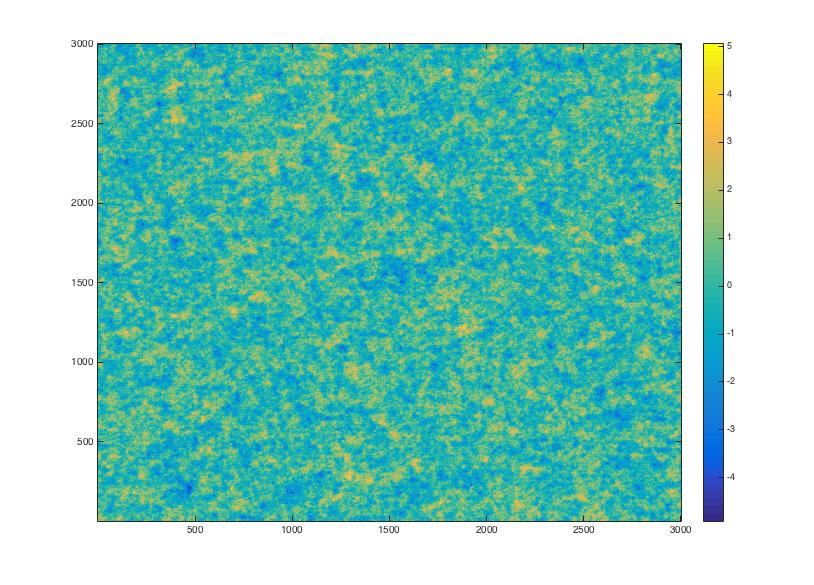
\includegraphics[width = 10cm]{ShadowFieldDeCorr20.jpg}
 \caption{Exponentially correlated shadowing field with $d_{0} = 20m$ (the color of the area refers to the normalized standard deviation, which is $S_{i}/\sigma_{s}(i)$)}

 \label{ch4:shadowingfield}
 \end{figure}

 Following the shadowing field generation algorithm, we generate shadowing fields with different de-correlation distances. A sample shadowing field is shown in Figure \ref{ch4:shadowingfield} with 20 meters de-correlation distance.

 \par Given a correlated shadowing field, the outage events at different locations are correlated. Without considering other small-scale fadings, the channel gain at different locations has a spatial correlation. An outage event occurs when SINR becomes less than $\gamma$, where $\gamma$ is a given SINR threshold. Based on the aforementioned correlated shadow fading model and the Random model, a correlated outage field can be generated as in Figure \ref{4:outagefie}. On the left, an outage field with independent log-normal shadow fading is shown, while the correlated outage field with correlated shadow fading is given on the right. The black color indicates outage areas. Outage areas due to the independent shadow fading are nonconsecutive dots. In contrast, those under the correlated shadow fading contain several connected areas . Therefore, we conclude that correlated shadow fading results in correlated outage areas with regard to the multi-cell system.

 \begin{figure*}
 \centering
 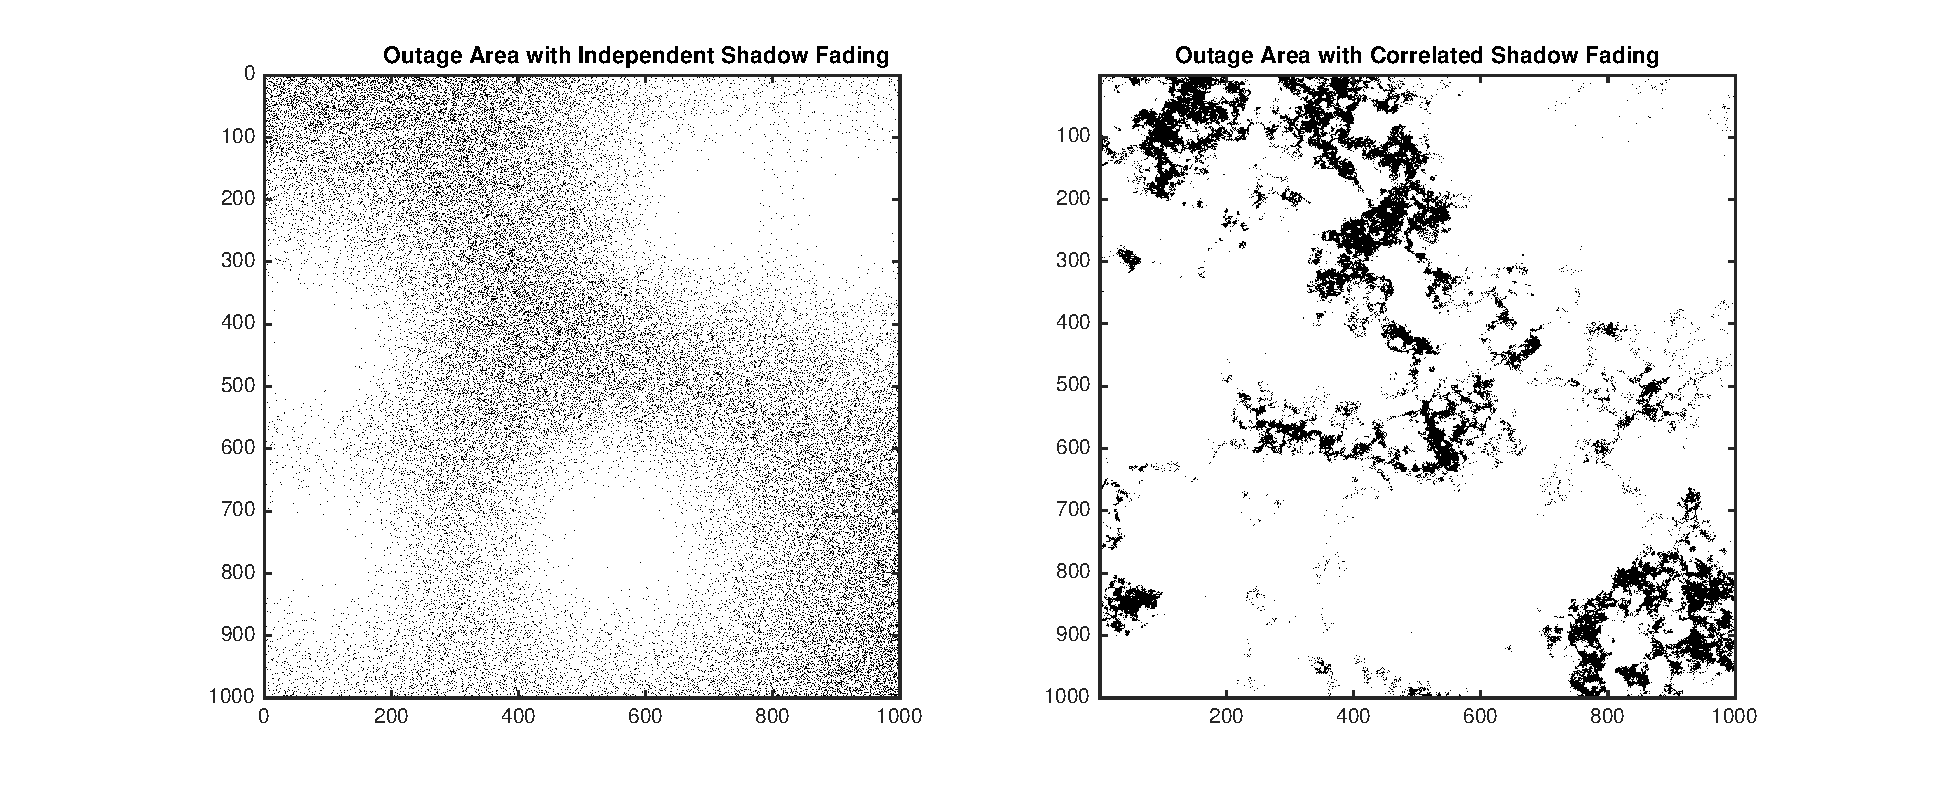
\includegraphics[width=14cm]{outageArea.eps}
 \caption{Correlated outage fields (Dark areas are outage areas while white areas are non-outage areas)}
 \label{4:outagefie}
 \end{figure*}


 \section{System Model}
 \label{4:SystemModel}
 In this section, we consider two system models with two different BS deployments: the Grid model and the Random model.
 \begin{itemize}
 \item Grid model: $\lambda$ BSs are placed on a regular grid deterministically.
 \item Random model: $\lambda$ BSs are placed randomly in a fixed area.
 \end{itemize}
 \begin{figure}
 \centering
 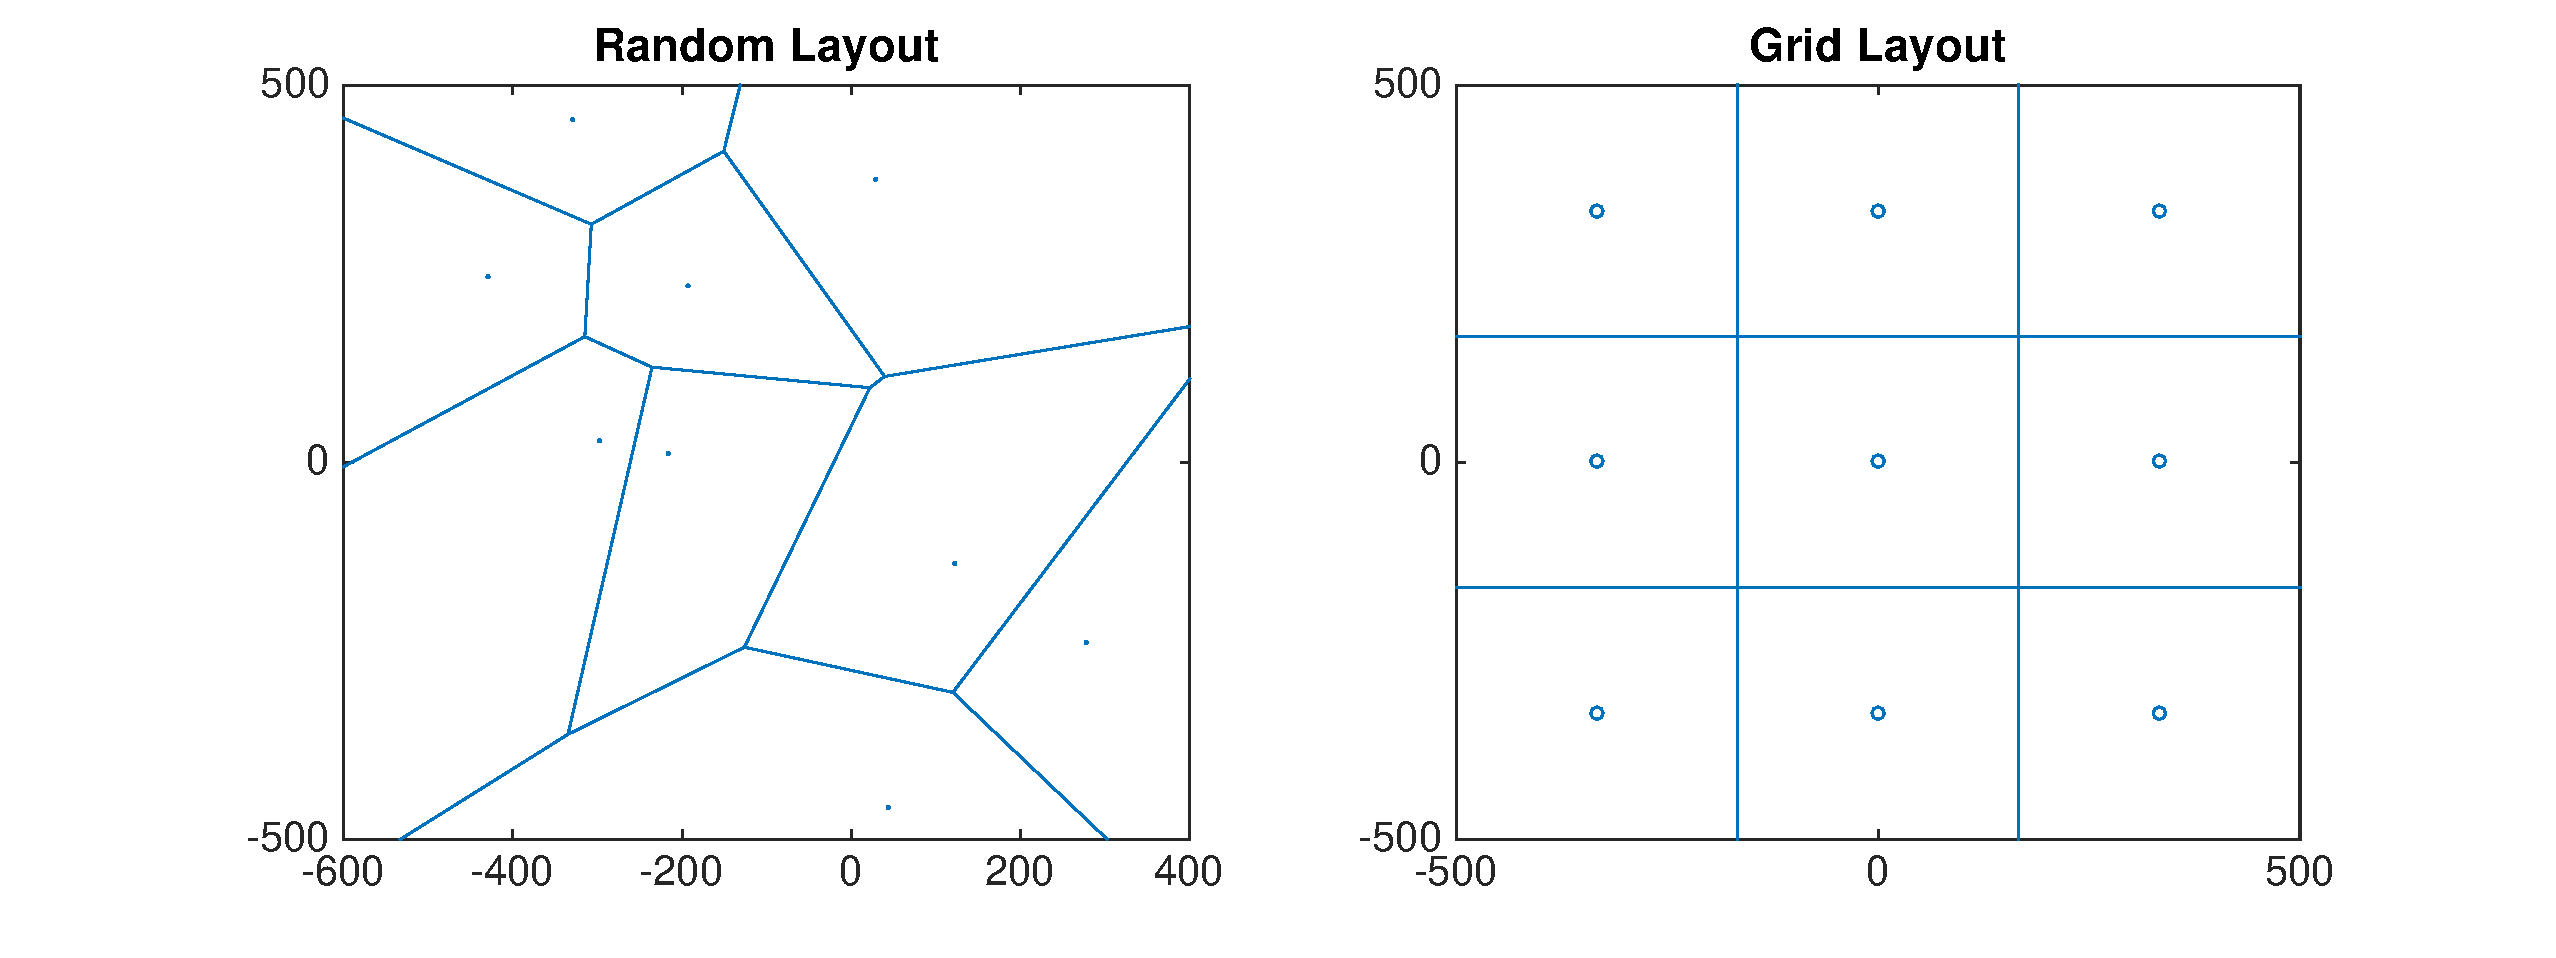
\includegraphics[width=14cm]{systemLayout.eps}
 \caption{Random model and Grid model with $\lambda = 9$.}
 \label{4:RandomLayout}
 \end{figure}
 % \begin{figure}
 % \centering
 % \includegraphics[width=8cm]{GridLayout.eps}
 % \caption{Grid Base Station Locations}
 % \label{GridLayout}
 % \end{figure}
\reminder{Give the figure an index, such as 4(a)} The left subfigure of Figure \ref{4:RandomLayout} is an example of the grid model, where cells are in regular square shape with the same size. For the Random model shown in the right subfigure, cells are not guaranteed to be the same shape or the same size. Distances between nearest base stations have a large variation from cell to cell


 \section{Outage Probability Analysis}
 \label{4:OutageProb}
 \par Let $\varphi = \{1, 2, \dots, N\}$ denotes the set of all BSs, then the received signal from BS $i$ to the destination user $D$ is given by:
 \begin{equation}
 y_{i\to D} = G_{i\to D}x_{i}+n_{D}.
 \end{equation}
 where $x_{i}$ is the signal transmitted by the source BS and $y_{i\to D}$ is the signal received by the destination user. $n_{D}\sim \mathcal{CN}(0,N_{0})$ is additive white Gaussian noise. $G_{i\to D}$ is the channel gain from source BS to MS including path loss and shadow fading. The end-to-end received $\text{SINR}$ is given in below:
 \begin{equation}
 \text{SINR} \triangleq \frac{P_{i}*G_{i\to D}^{2}}{N_{0}+\sum_{j\in \varphi/i}P_{j}*G_{j\to D}^2},
 \end{equation}
 where $P_{i}$ is the transmitted power of BS $i$. The MS successfully receives the signal if no outage event occurs, i.e., $\log_{2}(1+\text{SINR})\ge R$, where $R$ is the required data rate. From the definition of SINR, no outage event occurs as long as $\text{SINR} > \gamma$, where $\gamma = 2^{R}-1$.

 \par For a particular MS, outage event occurs when its received SINR is less than a threshold to decode the received signal. In our scenario, the probability that the receiver cannot decode signals received from its serving BS is defined as:
 \begin{equation}
 P(out_{i}) = P[\text{SINR}_{i\to D} < \gamma].
 \end{equation}
 We investigate two connection strategies: 
 \begin{itemize}
 \item Nearest BS: MS chooses to connect to the nearest BS.
 \item Strongest BS: MS chooses to connect to the BS providing highest SINR.
 \end{itemize}
 \par In the Nearest BS mode, we assume that the MS is served by the nearest BS, then the outage probability will be 
 \begin{equation}
 P_{out} = P_{out_{i}},
 \end{equation} 
 where $i$ is the index of the nearest BS. 
 \par In the Strongest BS mode, under the assumption that an MS is always connecting to the BS which provides the highest SINR, the outage event occurs if no BS can provide high enough SINR to the receiver. Based on this assumption we have:
 \begin{equation}
 P_{out} = \max_{i = 1,\cdots,N} P[\text{SINR}_{i\to D}<\gamma].
 \end{equation}
 The probability density function (pdf) of shadow fading $S$ given $L$ correlated fading branches is
 \begin{equation}
 \begin{split}
 f_{\mathbf{S}}(\mathbf{s}) = &\frac{\lambda^{L}}{\sqrt{2\pi}|\mathbf{K}_{L\times L}|^{1/2}\prod_{i=1}^{L}s_{i}}\\
 &\cdot\exp(-\frac{1}{2}(10\log_{10}\mathbf{s}-\boldsymbol{\mu})^{T}\mathbf{K}_{L\times L}^{-1}(10\log_{10}\mathbf{s}-\boldsymbol{\mu})),
 \end{split}
 \end{equation}
 where $\lambda = 10/\ln10$ and $\boldsymbol{\mu}$ is the average shadow fading which is normally $0$. $\mathbf{K}_{L\times L}$ is the correlation matrix which is defined in \eqref{correlationmatrix}. Let $\theta_{i} = \frac{10\log_{10}s_{i}-\mu_{i}}{\sqrt{2}\sigma_{i}}$, and doing a change of variables gives us the pdf of $\mathbf{\Theta}$ as follows:
 \begin{equation}
 f_{\mathbf{\Theta}}(\boldsymbol{\theta}) = \frac{1}{\pi^{L/2}|\mathbf{\Sigma}|^{1/2}}\exp(-\mathbf{\Theta}^{T}\mathbf{\Sigma}^{-1}\mathbf{\Theta}),
 \end{equation}
 where $\mathbf{\Sigma}$ is the correlation coefficient matrix which is
 \begin{equation}
 \left[\begin{array}{cccc}
 1 & h_{1,2} & \cdots & h_{1,L}\\
 \vdots & \ddots & \ddots & \vdots\\
 h_{L,1} & h_{L,2} & \cdots & 1\\
 \end{array}\right].
 \end{equation}
 Since $\text{SINR}_{i\to D}=PL_{i\to D}+S_{i}-N_{0}-\sum_{j\in\varphi/i}(PL_{j\to D} + S_{j})$ in dB, $\text{SINR}_{i\to D}<\gamma$ means
 \begin{equation}
 S_{i} - \sum_{j\in\varphi/i}S_{j}<\gamma -PL_{i\to D} + \sum_{j\in\varphi/i}PL_{j\to D} + N_{0},
 \end{equation}
 where $\varphi$ denotes the set of all BSs.
 Then the outage probability can be written as:
 \begin{equation}
 \label{4:outprob}
 P_{out} = \underbrace{\int_{-\infty}^{+\infty}\cdots\int_{-\infty}^{+\infty}}_{i =1,\cdots,N} g(PL_{i}S_{i} - \gamma\sum_{j\in\varphi/i}PL_{j}S_{j})f(\mathbf{s})d\mathbf{s},
 \end{equation}
 where $\mathbf{s}$ is the correlated shadow fading experienced by all BSs; $g(PL_{i}S_{i} - \gamma\sum_{j\in\varphi/i}PL_{j}S_{j})$ is a step function defined in (\ref{4:stepfunction}). 
%  \begin{figure}[!t]
% % ensure that we have normalsize text
% \normalsize
 % Store the current equation number.
 % \setcounter{MYtempeqncnt}{\value{equation}}
 % % Set the equation number to one less than the one
 % % desired for the first equation here.
 % % The value here will have to changed if equations
 % % are added or removed prior to the place these
 % % equations are referenced in the main text.

 \begin{equation}
 \label{4:stepfunction}
 g(PL_{i}S_{i} - \gamma\sum_{j\in\varphi/i}PL_{j}S_{j}) = \{\begin{array}{cc}
                1, &  \text{  when }PL_{i}S_{i} - \gamma\sum_{j\in\varphi/i}PL_{j}S_{j} <\frac{\gamma N_{0}}{P}\\
                0, & \text{  when }PL_{i}S_{i} - \gamma\sum_{j\in\varphi/i}PL_{j}S_{j} >\frac{\gamma N_{0}}{P}
              \end{array}.
 \end{equation}
 % Restore the current equation number.
 % \setcounter{equation}{\value{MYtempeqncnt}}
 % IEEE uses as a separator
% \hrulefill
% % The spacer can be tweaked to stop underfull vboxes.
% \vspace*{4pt}
% \end{figure}

 \section{Simulation Results}
 \label{4:SimuProb}
 \par In this section, we present simulation setup and results. Firstly, we execute simulations to compare the outage probability of the two different network topologies: the Grid model and the Random model. Secondly, the SINR distribution and the outage probability of the Random model given different BS densities are investigated. Two scenarios are considered: MS connecting to the nearest BS and MS connecting to the BS providing highest SINR. At the end, the outage duration distribution is simulated and discussed given different BS densities. The simulation parameters are presented in Table \ref{SystemConfig2}. 
 \begin{table}
 \centering
 \caption{\label{SystemConfig2}Simulation Configuration Parameters}

 \begin{tabular}{|c|c|}

 \hline
 Target Area & $1000m\times 1000m$\\
 \hline
 BS Densities & $3, 10, 50, 100, 200, 300, 500$\\
 \hline
 Path Loss Exponent & $4$\\
 \hline
 BS Transmission Power & $P: 40dbm$\\
 \hline
 SINR Requirement & $-5dB$\\
 \hline
 De-Correlation Distance & $20m, 200m$\\
 \hline
 \end{tabular}

 \end{table}

 \par Figure \ref{4:cdf1} shows the Cumulative Distribution Function (CDF) of SINR when the MS is connecting to the nearest BS. The de-correlation distance of the correlated shadow fading is $20m$. The figure suggests that the Grid model outperforms the Random model, which is consistent with findings in \cite{andrews2011tractable}. Figure \ref{4:outage1} shows the outage probability with SINR threshold being $-5dB$. The outage probability of Grid model (blue) is lower than that of the Random model (yellow). In the next section, we will focus on the Random model, which is more realistic than the Grid model.
 \begin{figure}
 \centering
 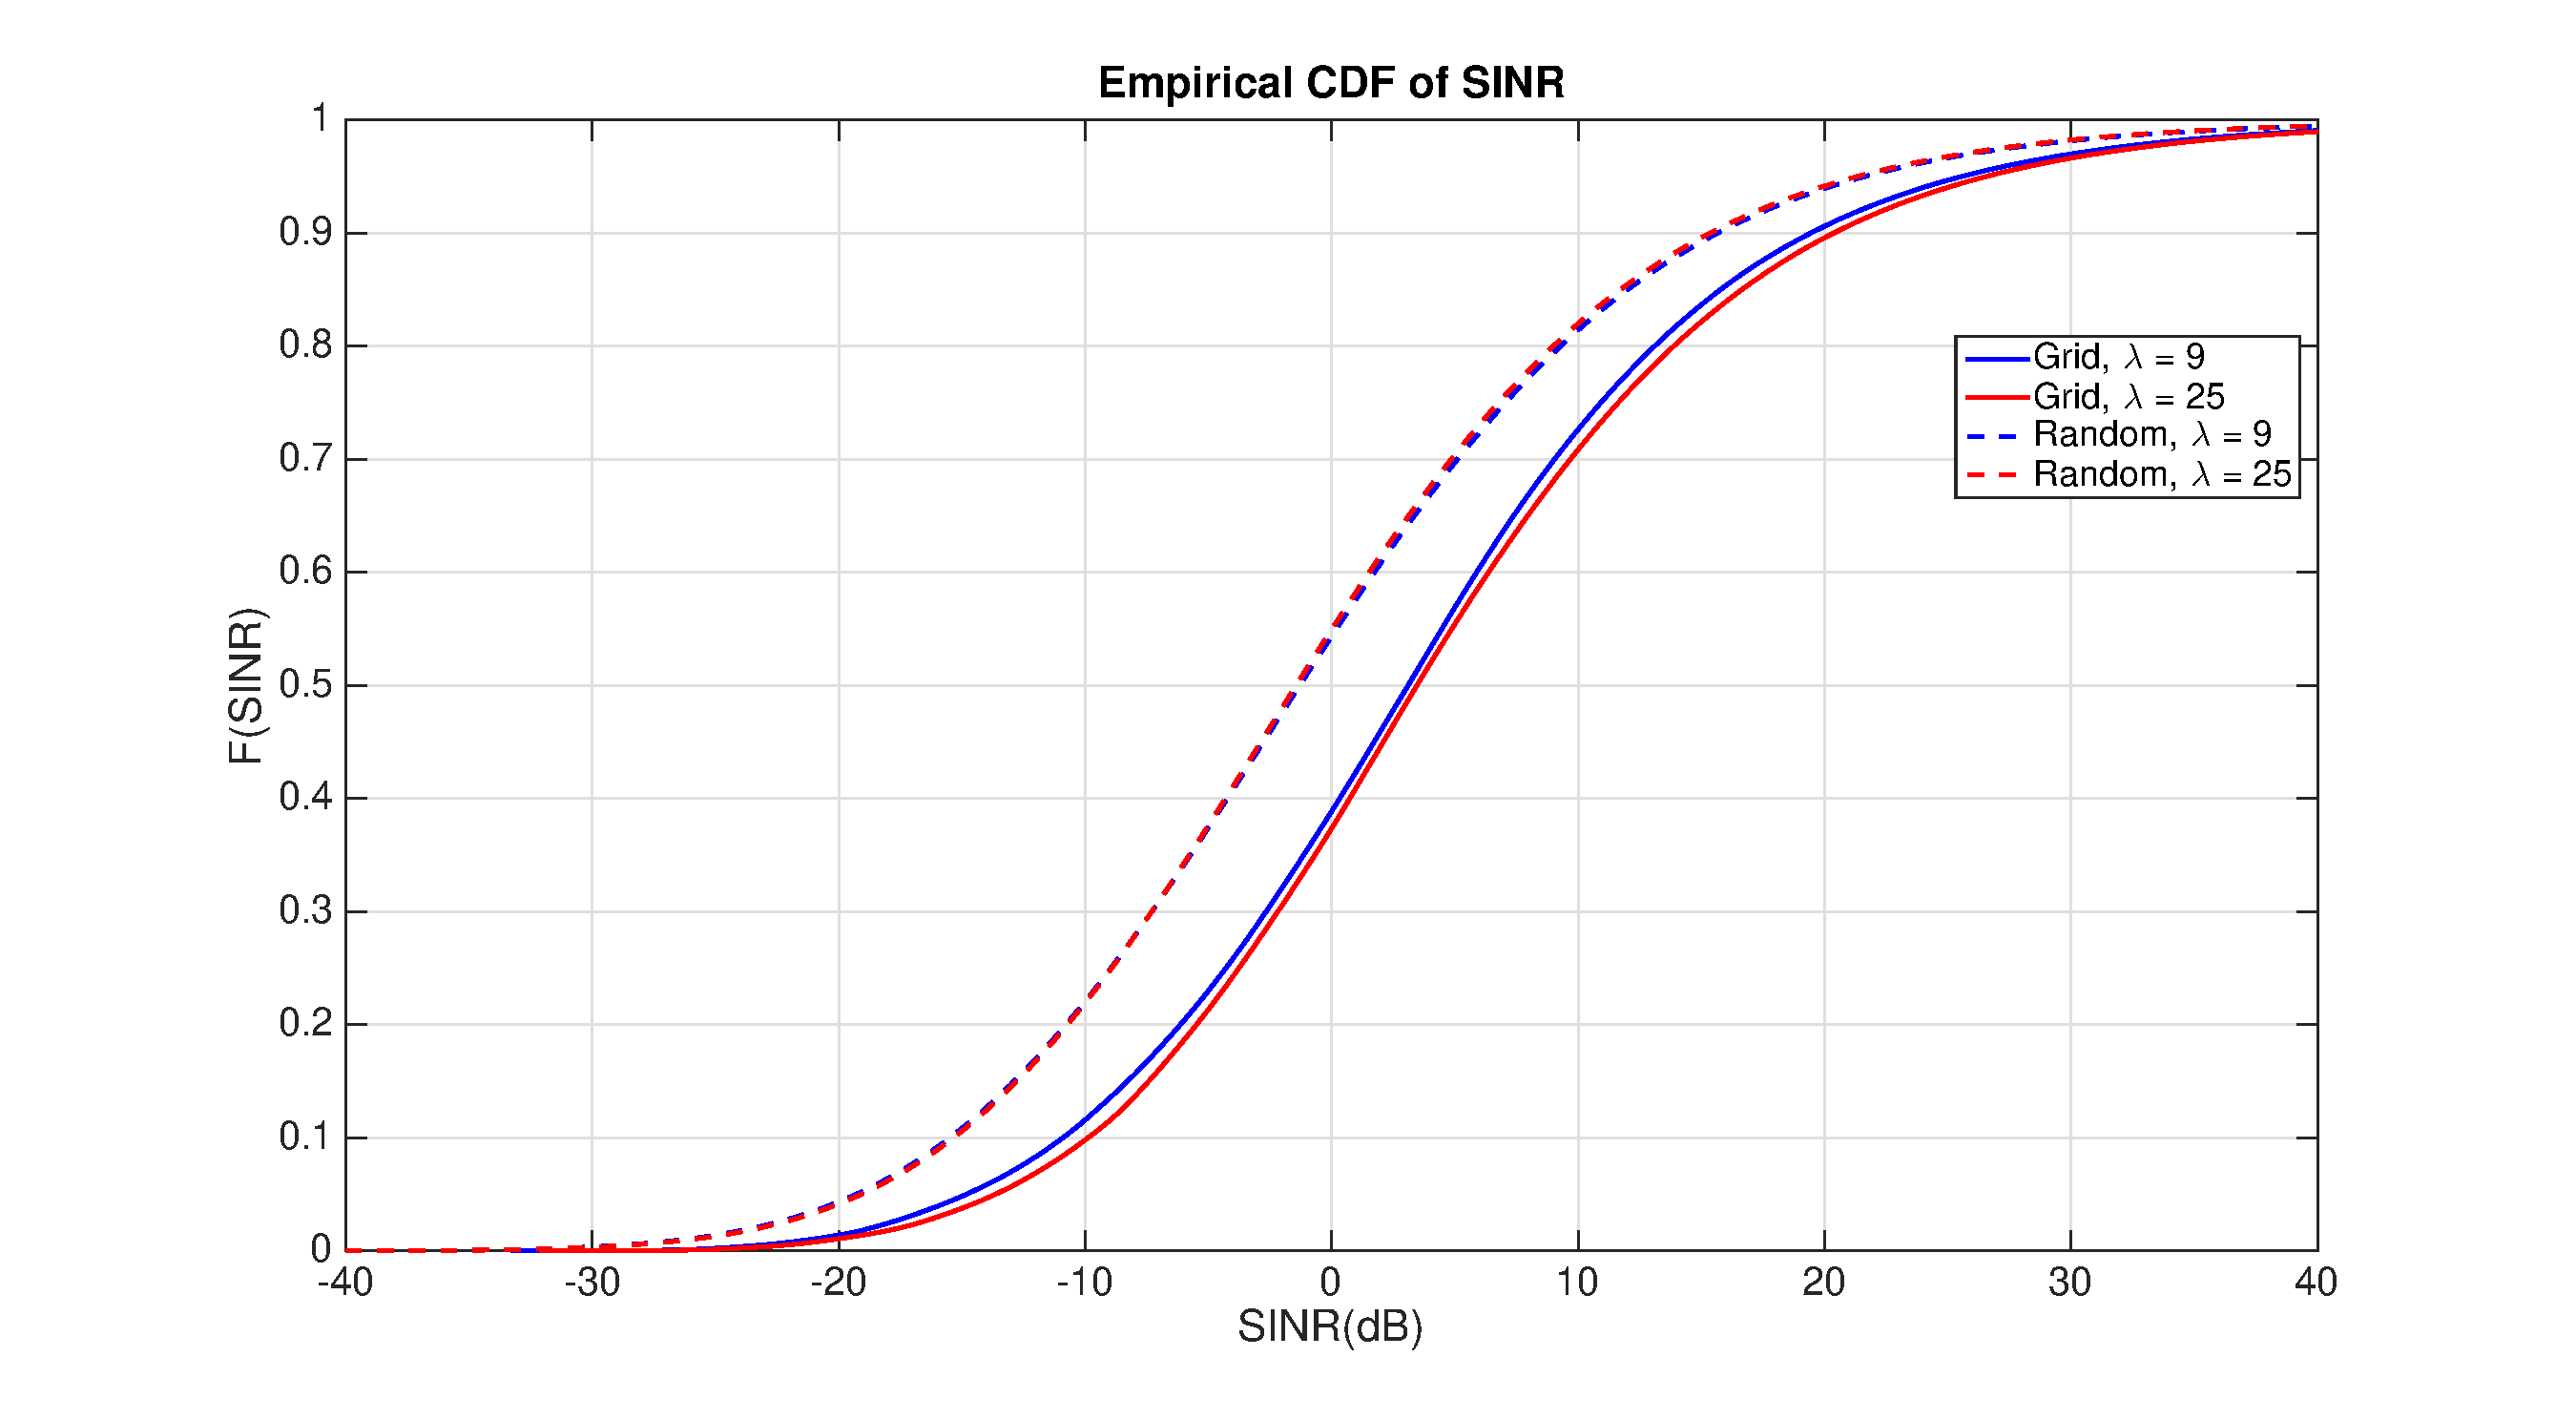
\includegraphics[width=10cm]{GridVSRandom.eps}
 \caption{CDF of SINR given Grid model and Random model (de-correlation distance: $20m$)}
 \label{4:cdf1}
 \end{figure}
 \begin{figure}
 \centering
 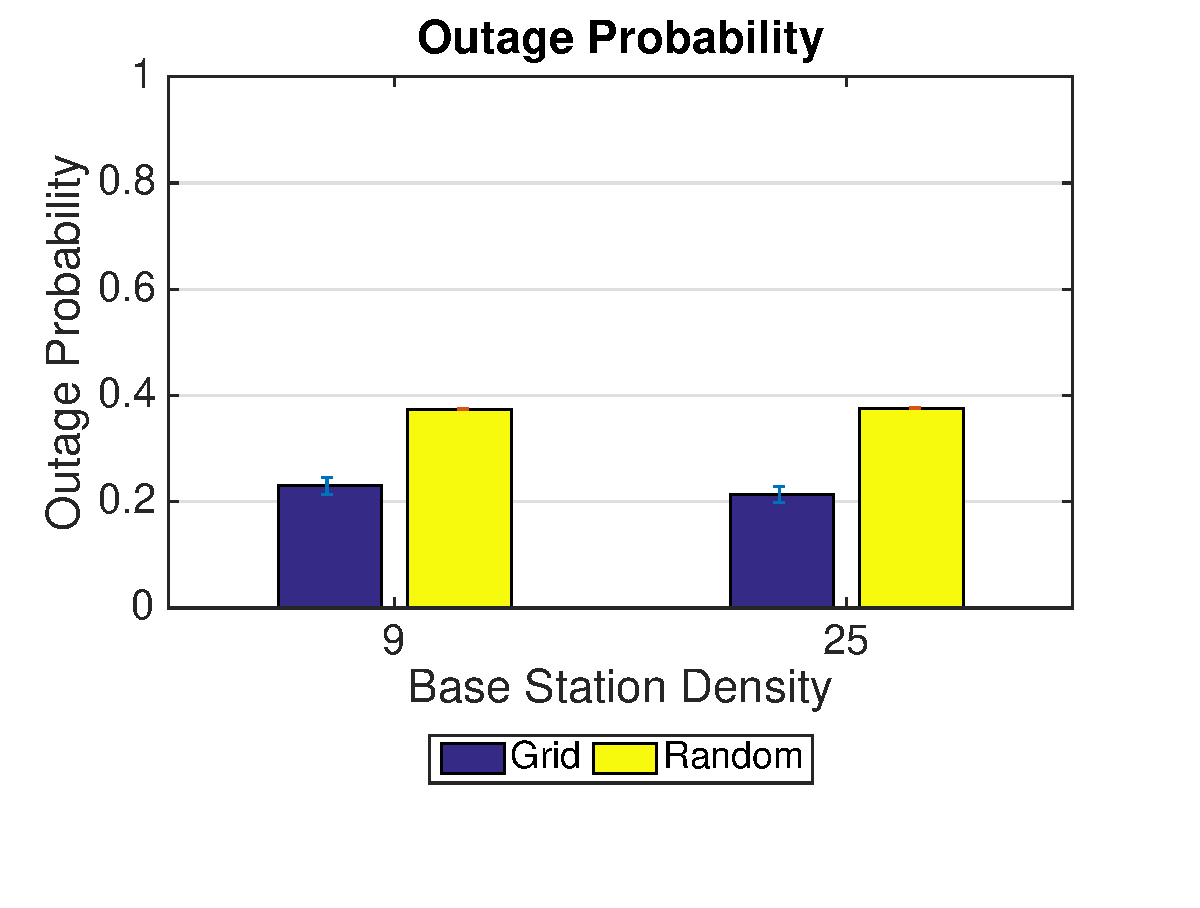
\includegraphics[width=10cm]{OutageProbGridVSRandom.eps}
 \caption{Outage probability given Grid model and Random model with $\gamma = -5dB$ (de-correlation distance: $20m$)}
 \label{4:outage1}
 \end{figure}


 \begin{figure}
 \centering
 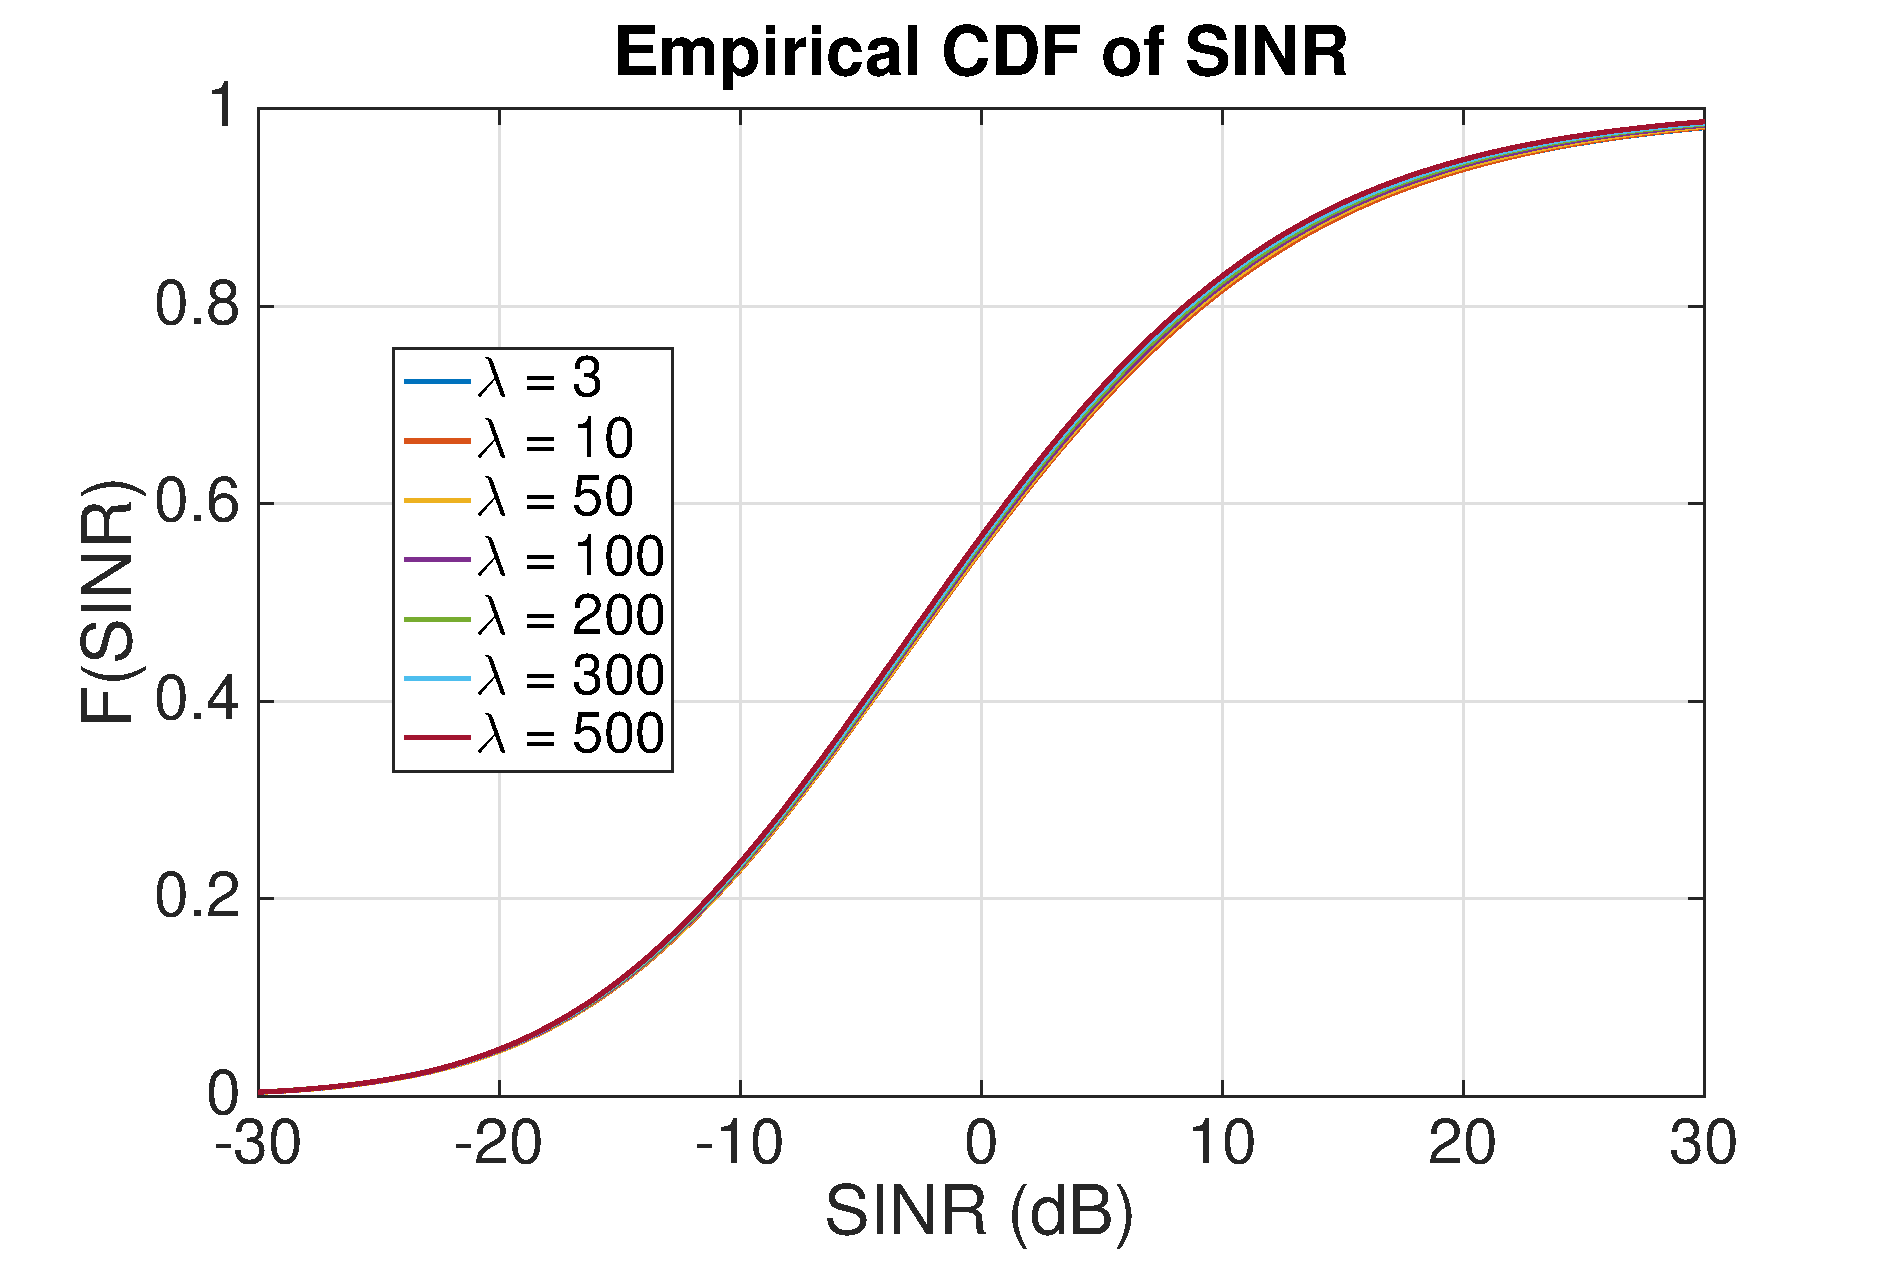
\includegraphics[width=10cm]{NBMax1000OutageProbCDFiid.eps}
 \caption{CDF of SINR (the MS is connecting to the nearest BS, independent shadow fading}
 \label{4:Mode1}
 \end{figure}
 \begin{figure}
 \centering
 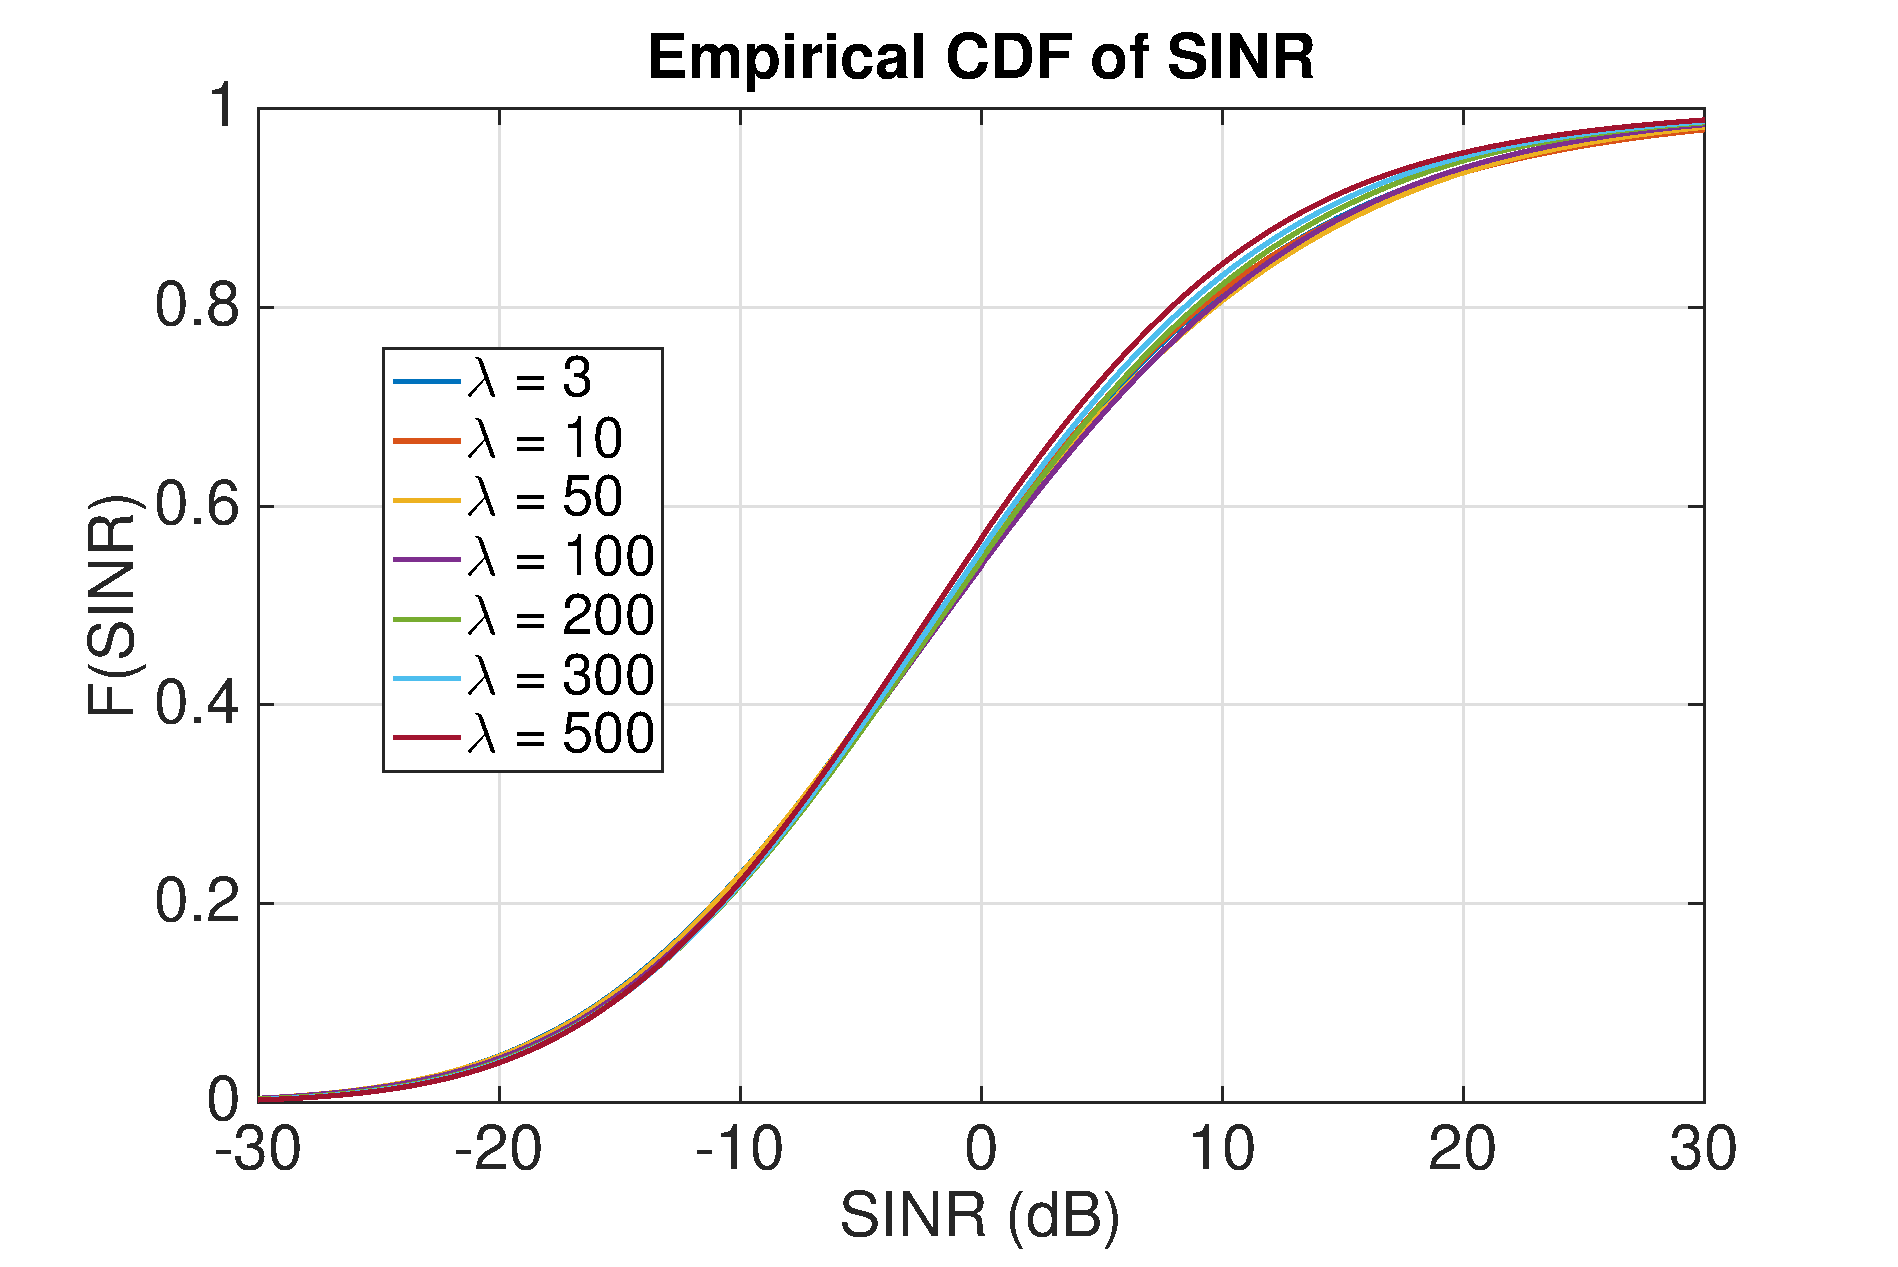
\includegraphics[width=10cm]{NBMax1000OutageProbCDFDeCorr20.eps}
 \caption{CDF of SINR (the MS is connecting to the nearest BS, correlated shadow fading with 20m de-correlation distance}
 \label{4:Mode2}
 \end{figure}
 \begin{figure}
 \centering
 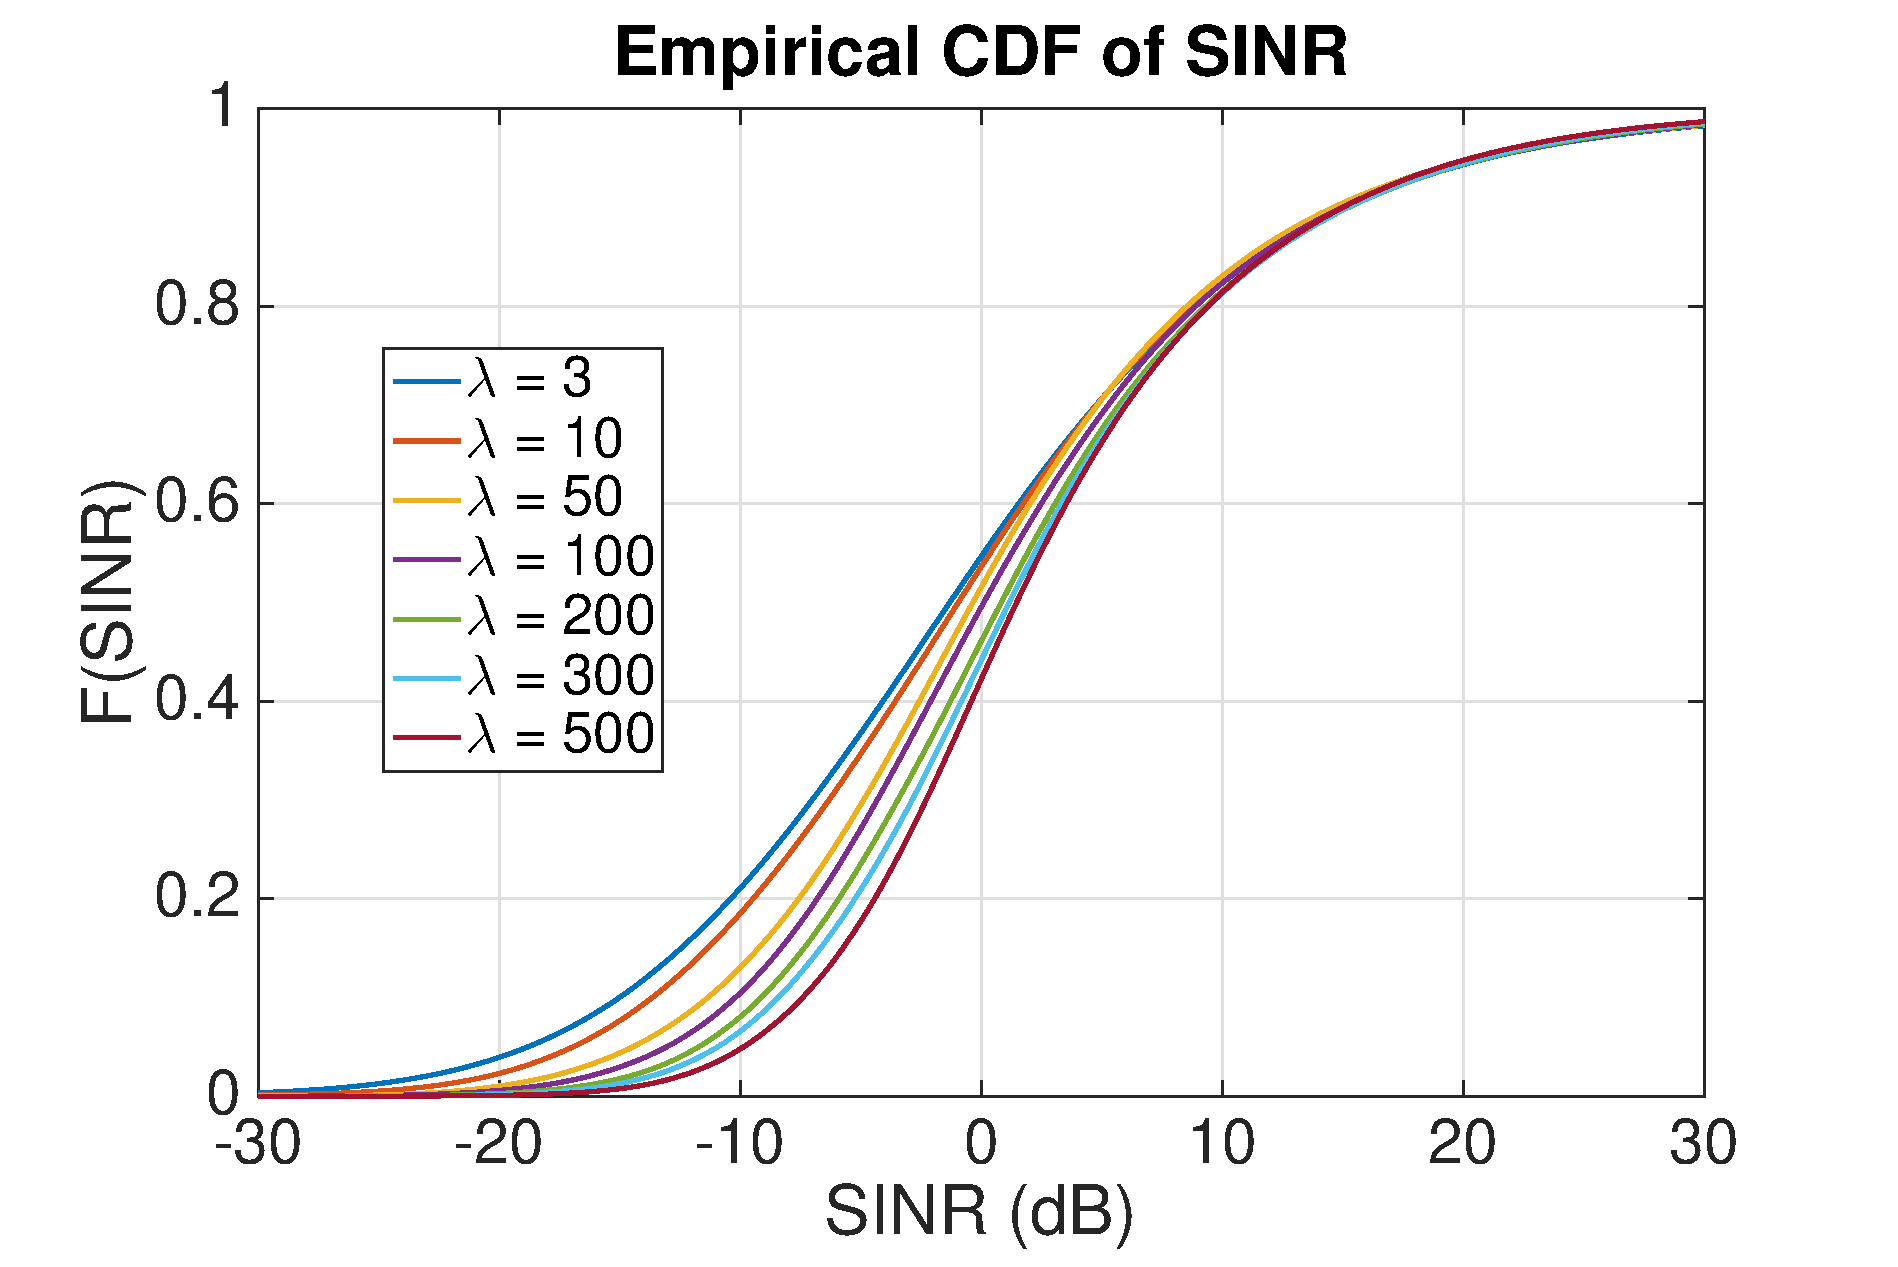
\includegraphics[width=10cm]{NBMax1000OutageProbCDFDeCorr200.eps}
 \caption{CDF of SINR (the MS is connecting to the nearest BS, correlated shadow fading with 200m de-correlation distance}
 \label{4:Mode3}
 \end{figure}


 \begin{figure}
 \centering
 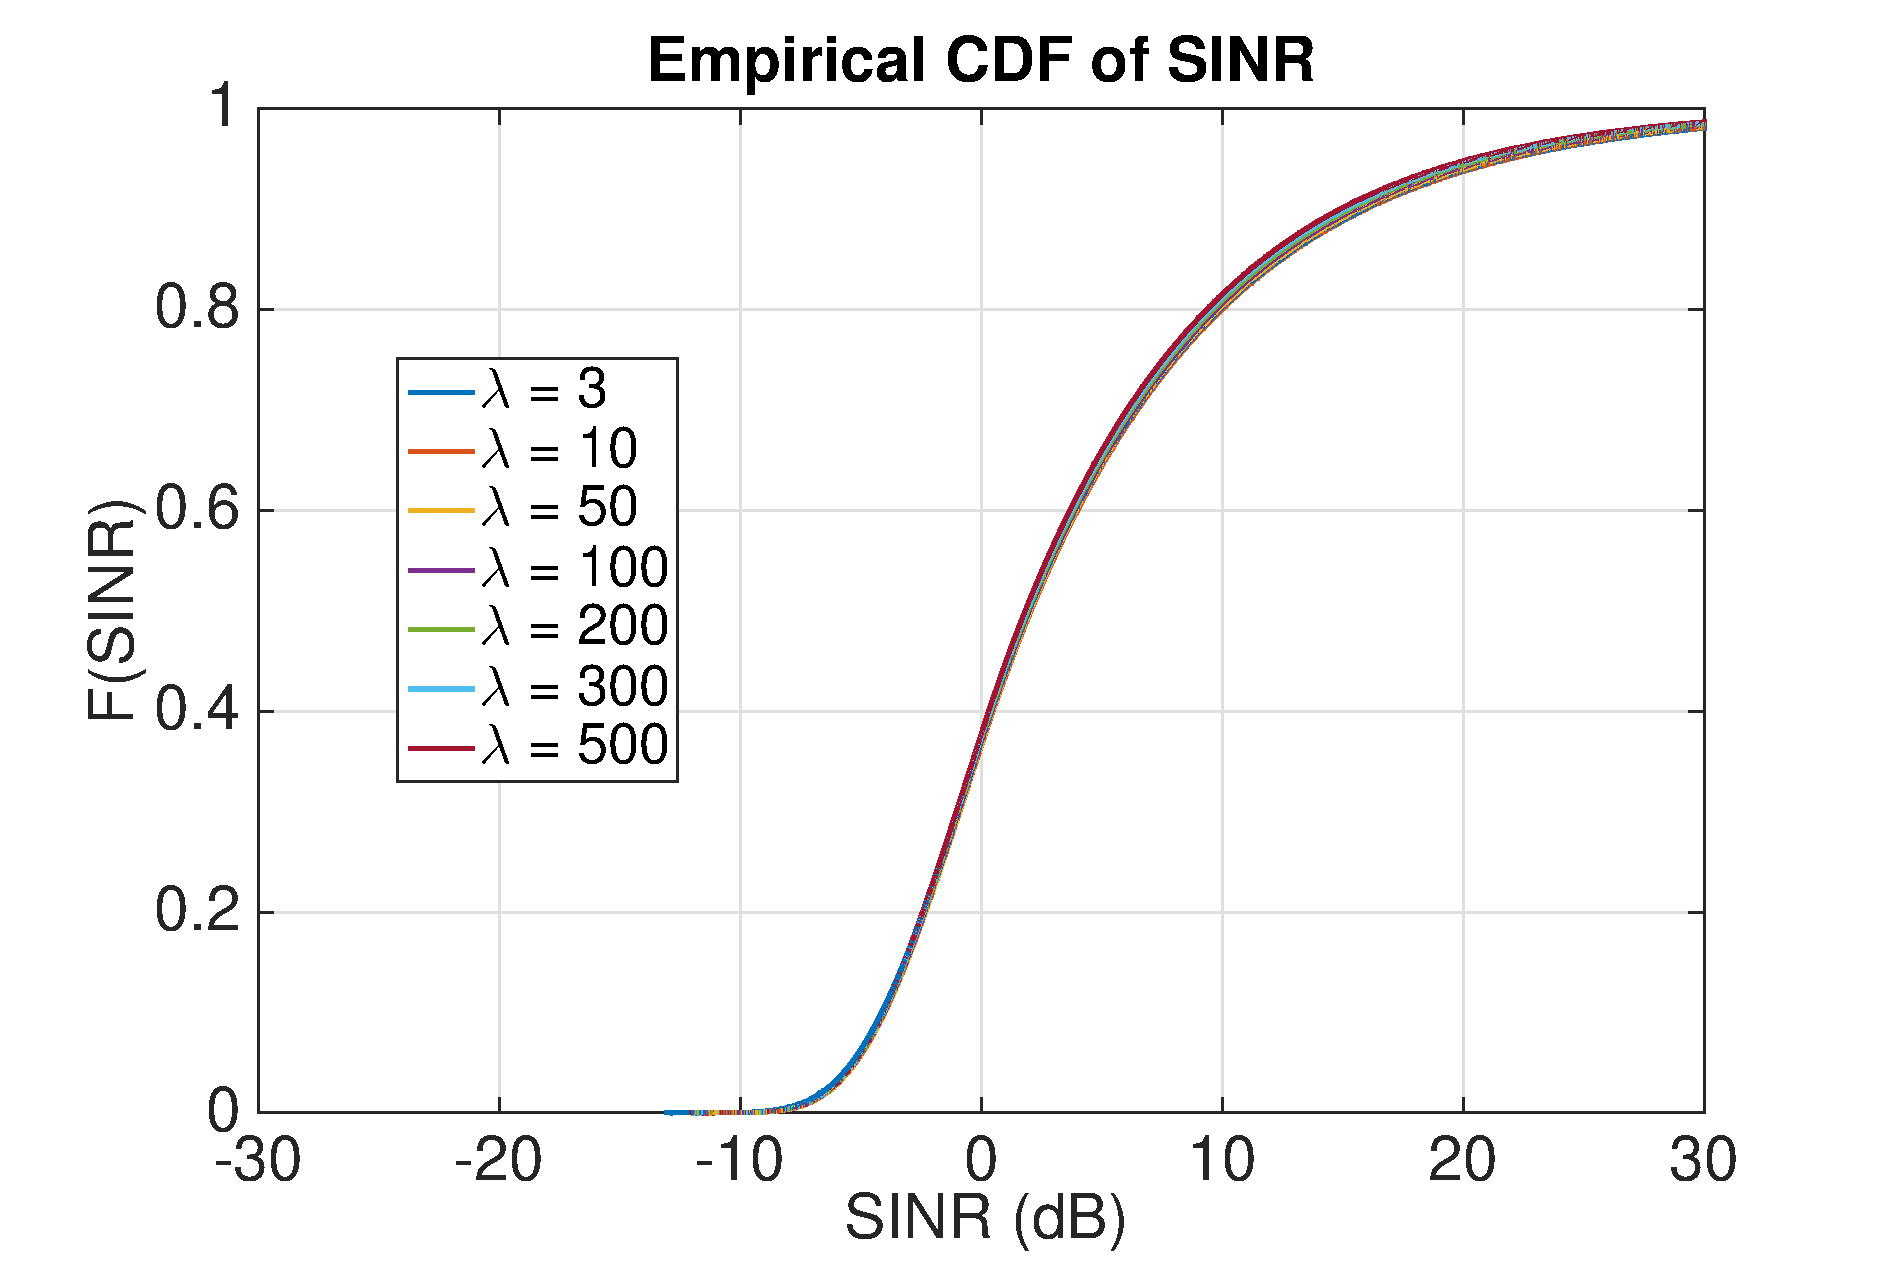
\includegraphics[width=10cm]{MaxMax1000OutageProbCDFiid.eps}
 \caption{CDF of SINR (the MS is connecting to the strongest BS, independent shadow fading}
 \label{4:Mode12}
 \end{figure}
 \begin{figure}
 \centering
 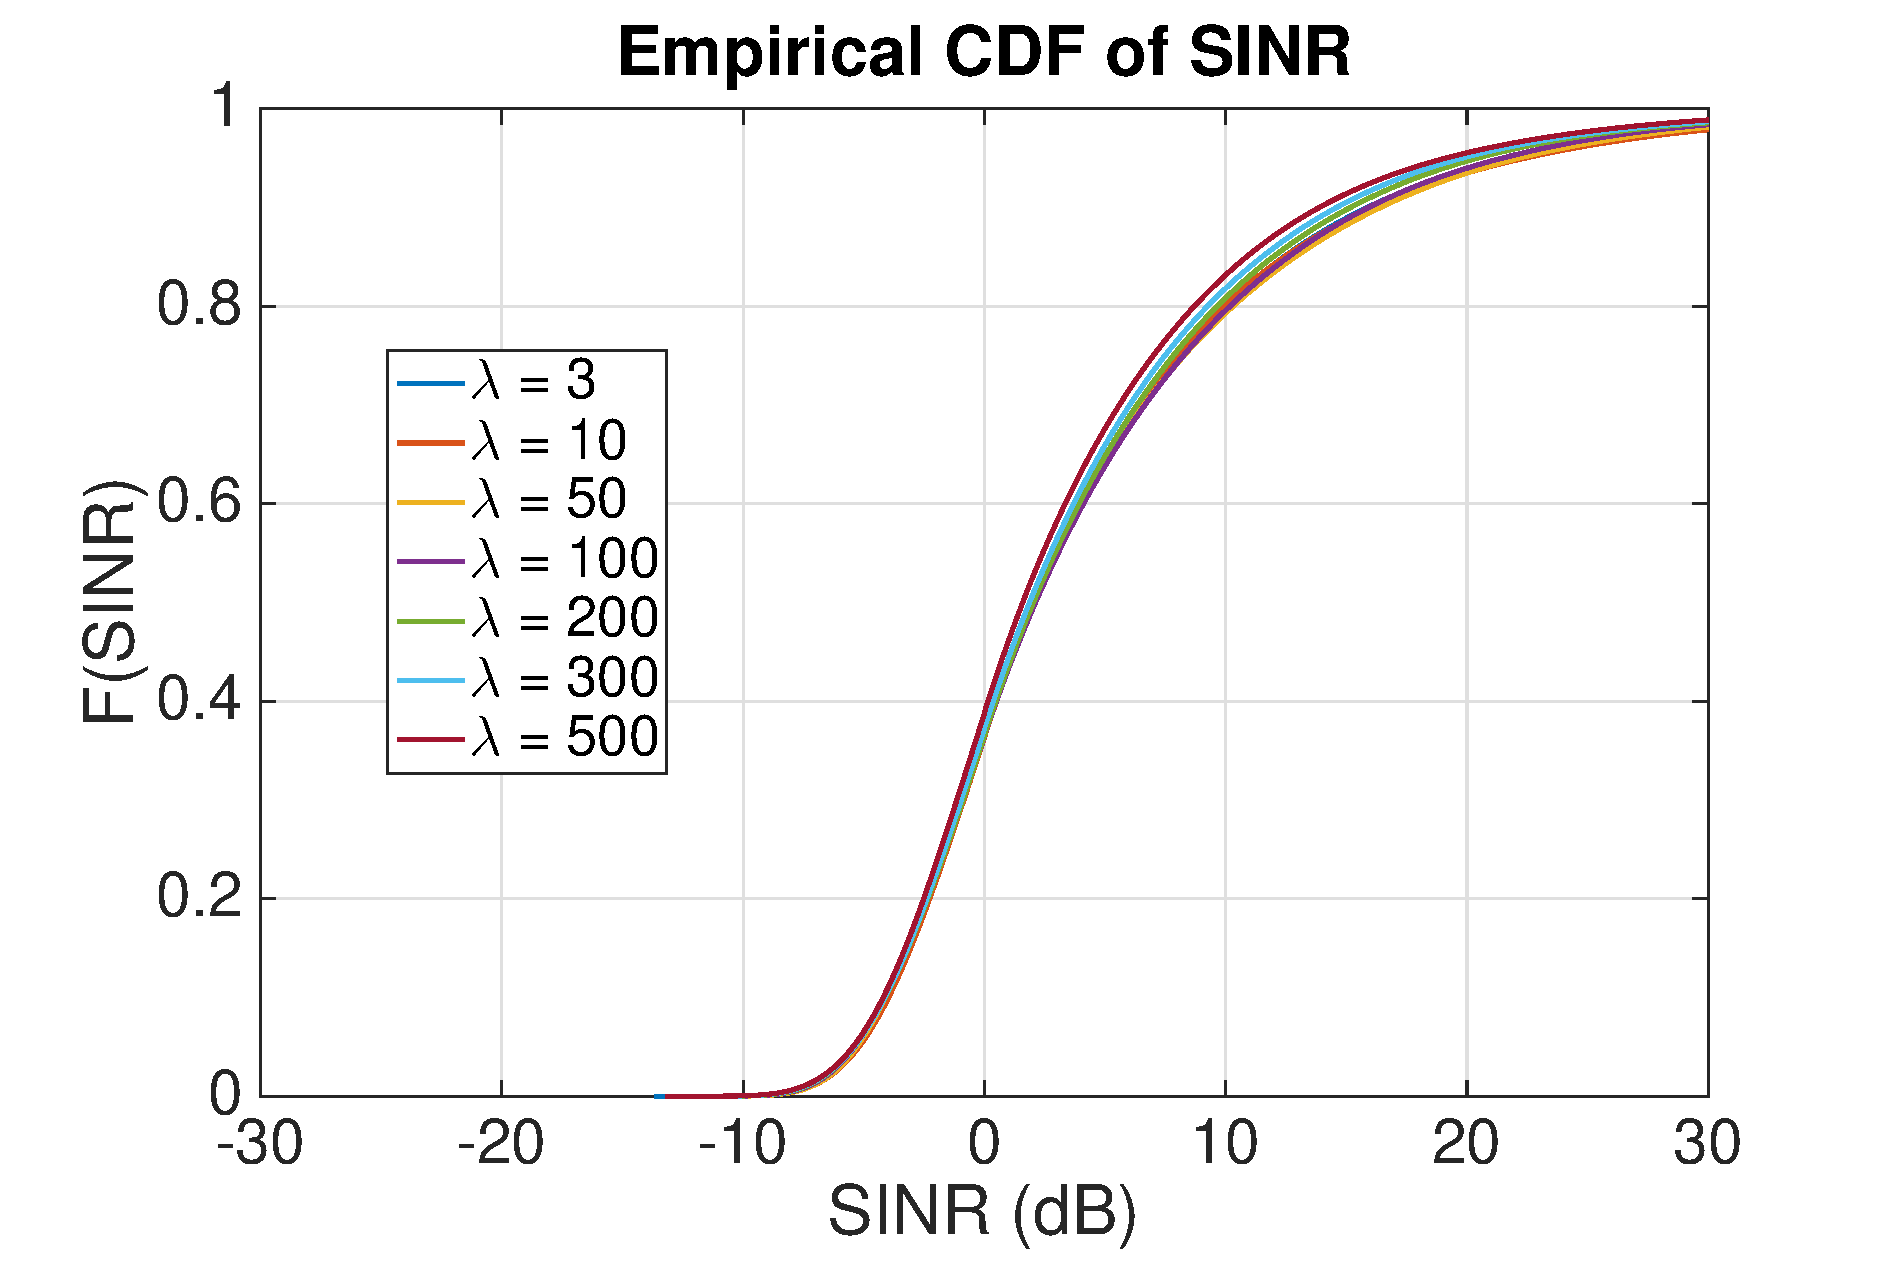
\includegraphics[width=10cm]{MaxMax1000OutageProbCDFDeCorr20.eps}
 \caption{CDF of SINR (the MS is connecting to the strongest BS, correlated shadow fading with 20m de-correlation distance}
 \label{4:Mode22}
 \end{figure}
 \begin{figure}
 \centering
 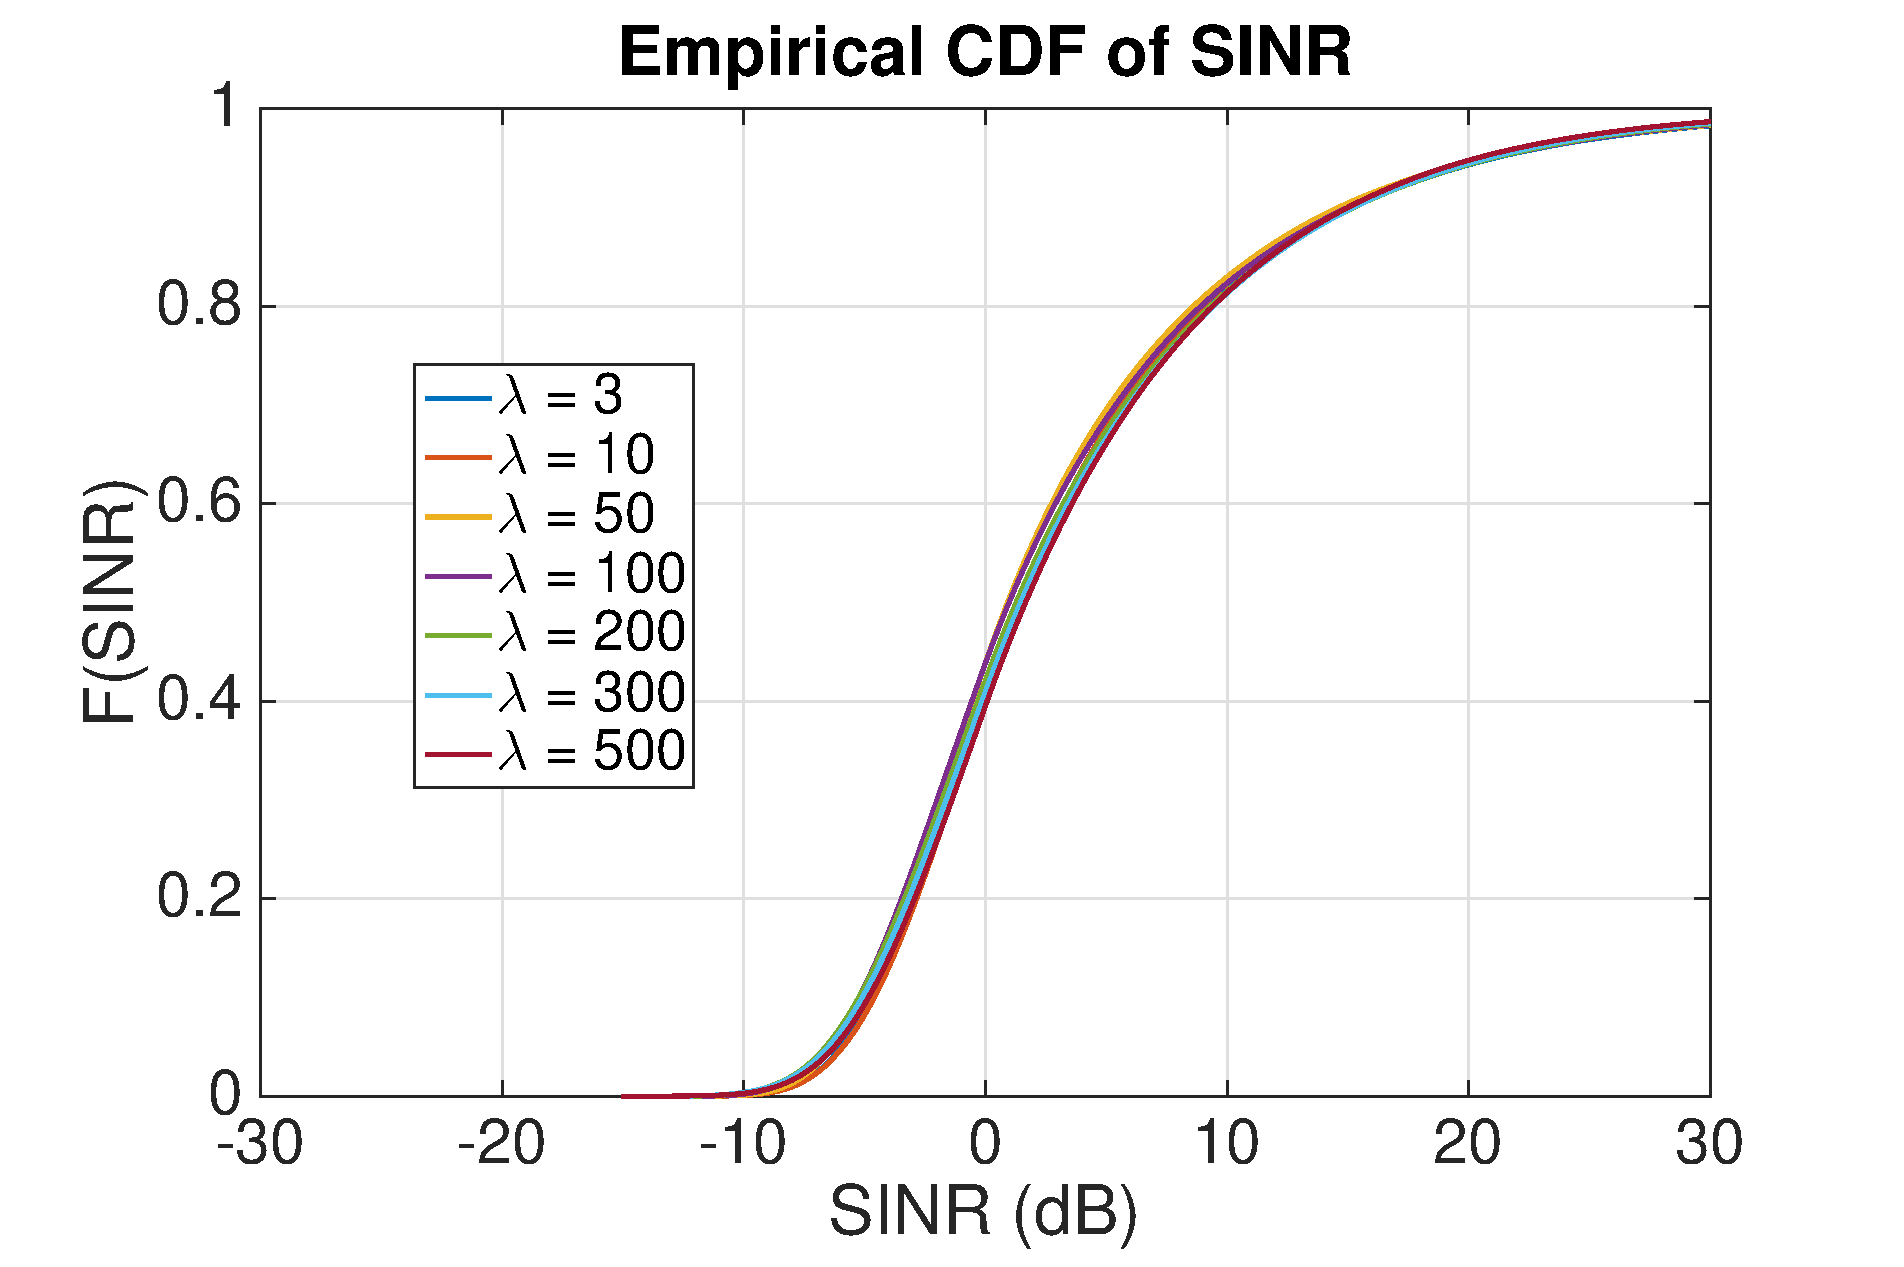
\includegraphics[width=10cm]{MaxMax1000OutageProbCDFDeCorr200.eps}
 \caption{CDF of SINR (the MS is connecting to the strongest BS, correlated shadow fading with 200m de-correlation distance}
 \label{4:Mode32}
 \end{figure}

 \par For the Random model, the SINR distribution and the outage probability of different BS densities are investigated for both the Nearest BS mode and the Strongest BS mode. Simulations are implemented under independent shadow fading and correlated shadow fading. CDF curves of SINR are generated and the outage probability given the SINR threshold being $-5dB$ are presented for increasing BS densities. Figure \ref{4:Mode1}, \ref{4:Mode2} and \ref{4:Mode3} show the SINR of the MS when connecting to the nearest BS. From Figure \ref{4:Mode1} and \ref{4:Mode2}, it is obvious that the CDF curves are overlapping each other, which means increasing BS density does not change the CDF of SINR. From this we can conclude, under the circumstance that the shadow fading is independent or the de-correlation distance of the correlated shadow fading is small, increasing the BS density will not improve the system performance in terms of reducing the outage probability. Figure \ref{4:Mode3}  illustrates that CDF of SINR improves (curve moves toward the bottom-right corner) as we increase the BS density. Therefore, increasing the BS density will result in better system performance when the de-correlation distance is large, by reducing the outage probability. Figure \ref{fig: outprob1} shows the outage probability of different correlated shadow fading models and different BS densities when SINR threshold is set to $-5dB$. These blue and green bars suggest that increasing the BS density will not decrease the outage probability when shadow fading is independent or correlated with $20m$ de-correlation distance. Meanwhile, these yellow bars suggest that when the de-correlation distance is $200m$, increasing the BS density will reduce the outage probability. For example, when the BS density is $3$, the outage probability is around $38\%$. Increasing the BS density to $500$, the outage probability decreases to $18\%$. Above simulation results suggest that when the de-correlation distance is relatively large and the MS is connecting to the nearest BS, increasing the BS density will reduce the outage probability and improve the system performance.



 \begin{figure}
 \centering
 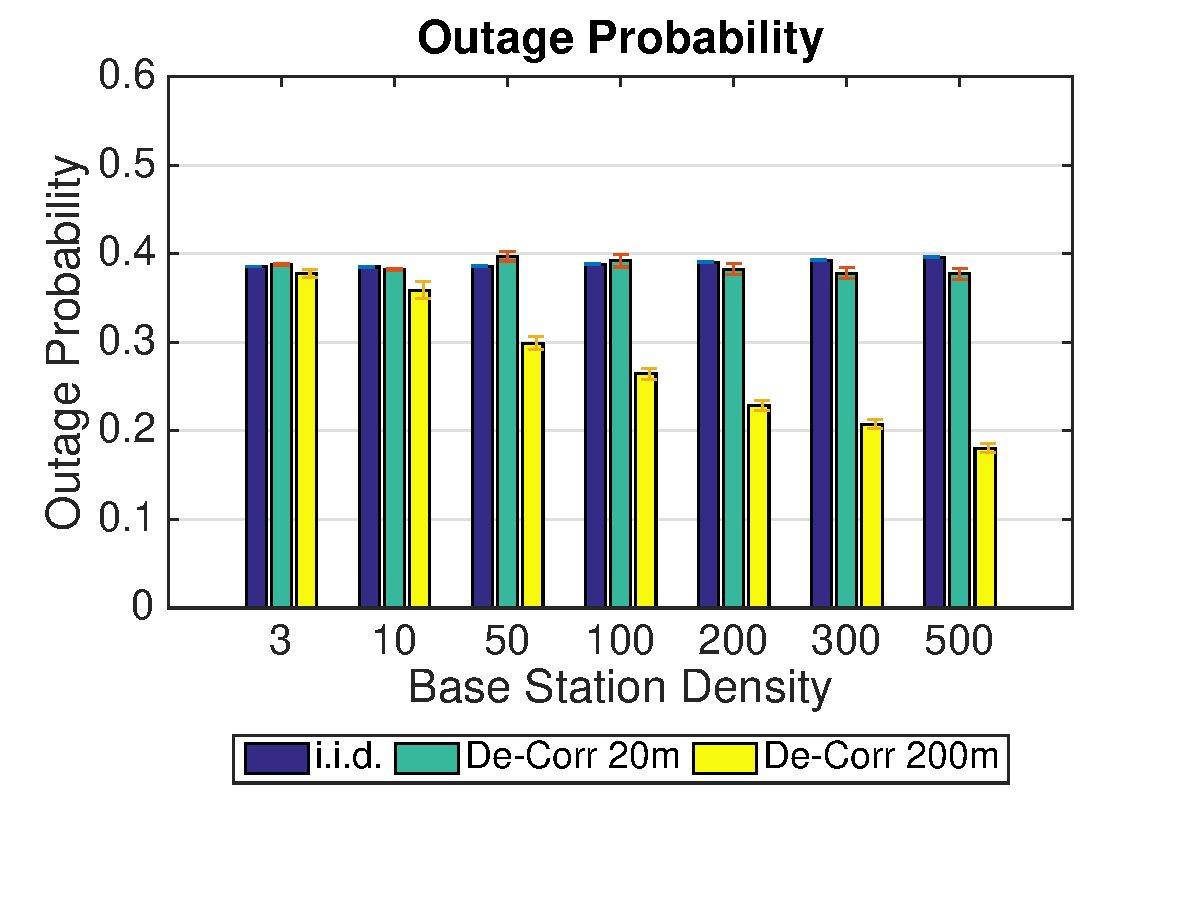
\includegraphics[width=10cm]{NBMax1000OutageProbThresh-5iid.eps}
 \caption{Outage probability given $-5dB$ SINR threshold}
 \label{fig: outprob1}
 \end{figure}
 \begin{figure}
 \centering
 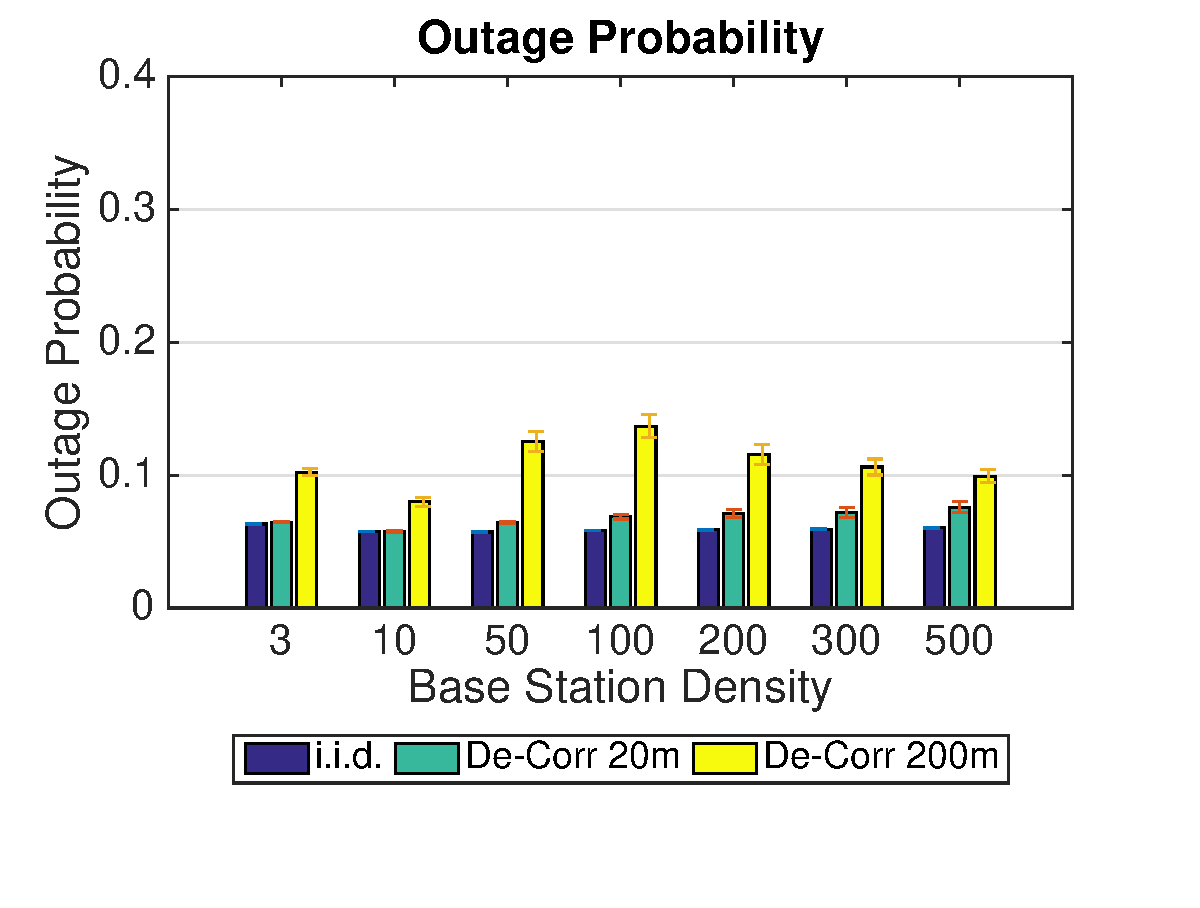
\includegraphics[width=10cm]{MaxMax1000OutageProbThresh-5iid.eps}
 \caption{Outage probability given $-5dB$ SINR threshold}
 \label{fig: outprobs2}
 \end{figure}
 \begin{figure}
 \centering
 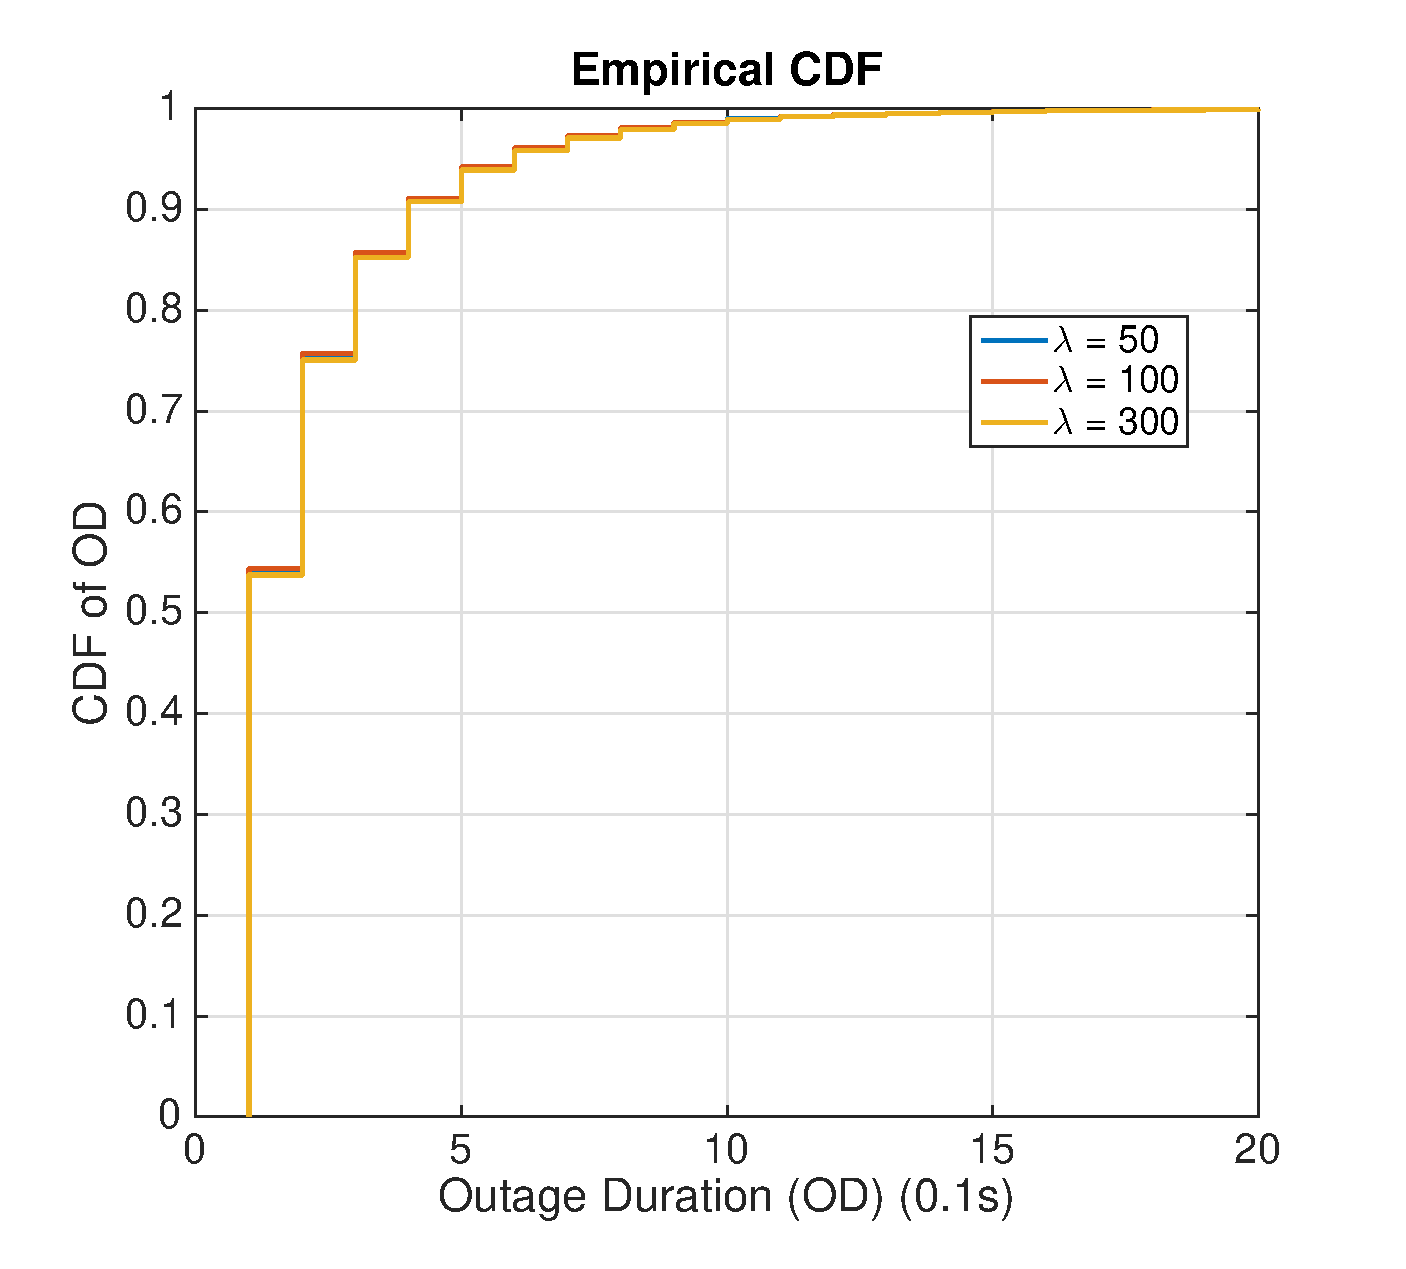
\includegraphics[width=10cm]{ODthresh-5iidNB.eps}
 \caption{CDF of Outage Durations when the MS is connecting to the Nearest BS with independent shadow fading}
 \label{iid1}
 \end{figure}
 \begin{figure}
 \centering
 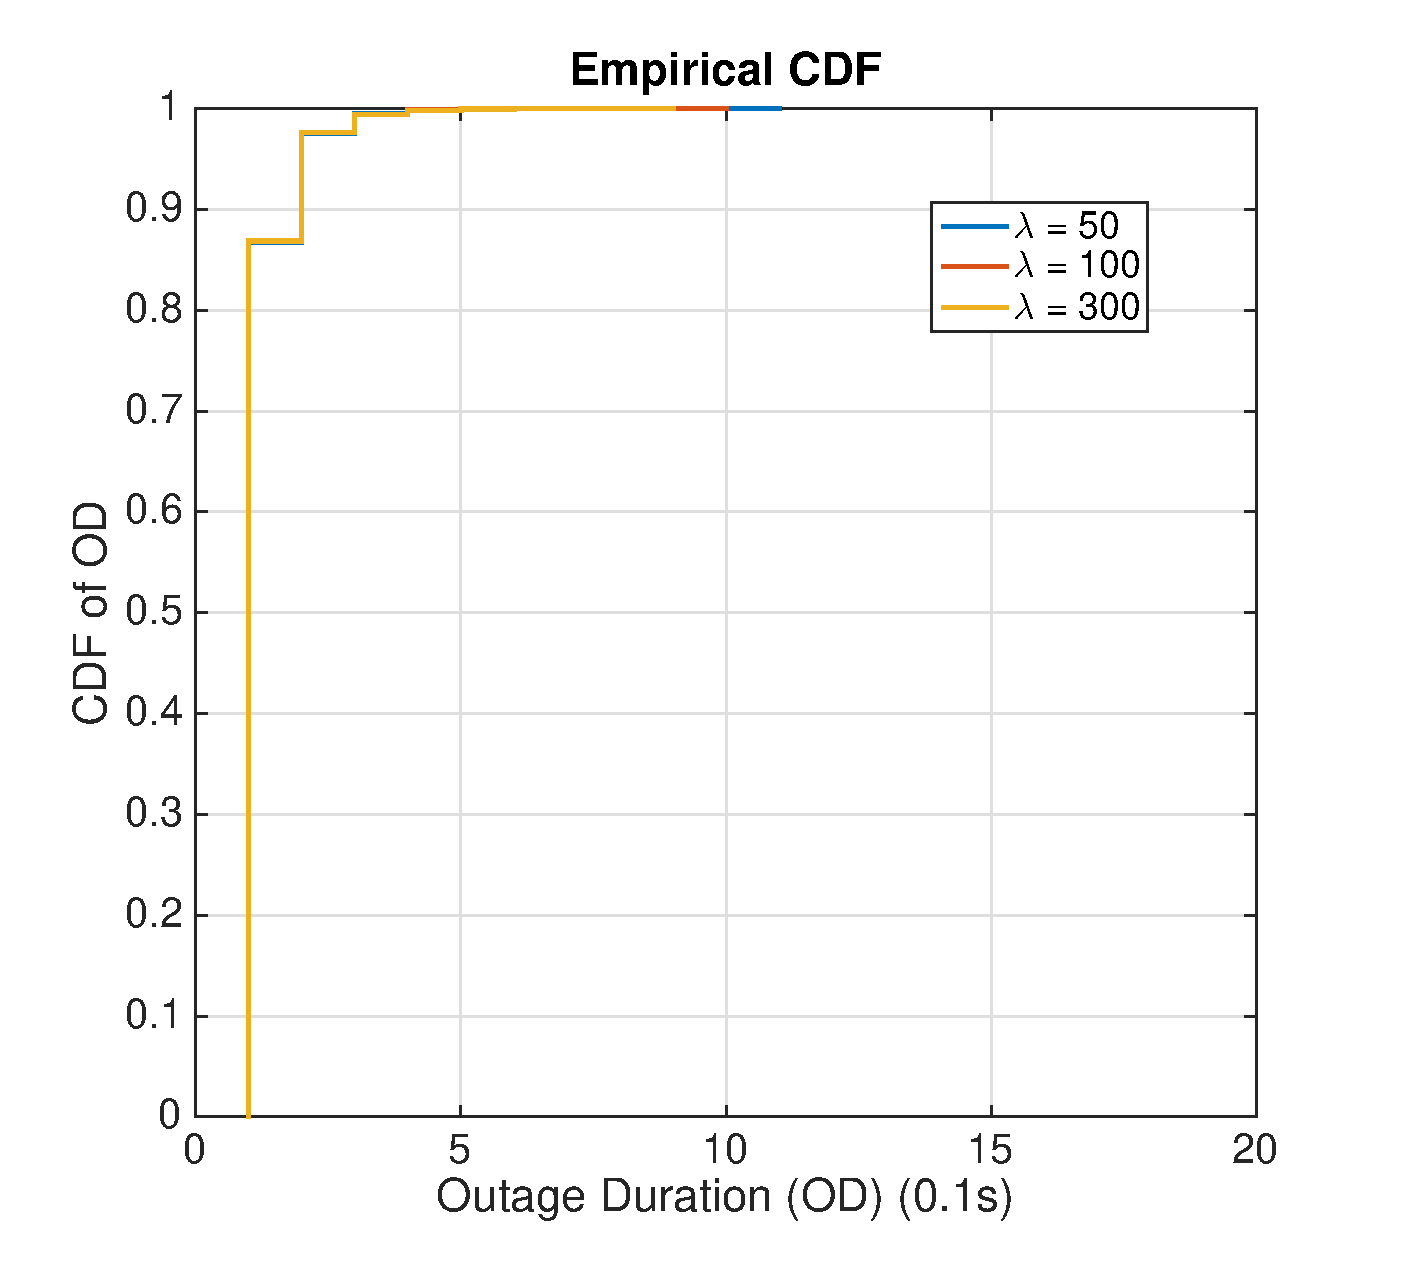
\includegraphics[width=10cm]{ODthresh-5iidMax.eps}
 \caption{CDF of Outage Durations when the MS is connecting to the Strongest BS with independent shadow shadowing}
 \label{iid2}
 \end{figure}
 \begin{figure}
 \centering
 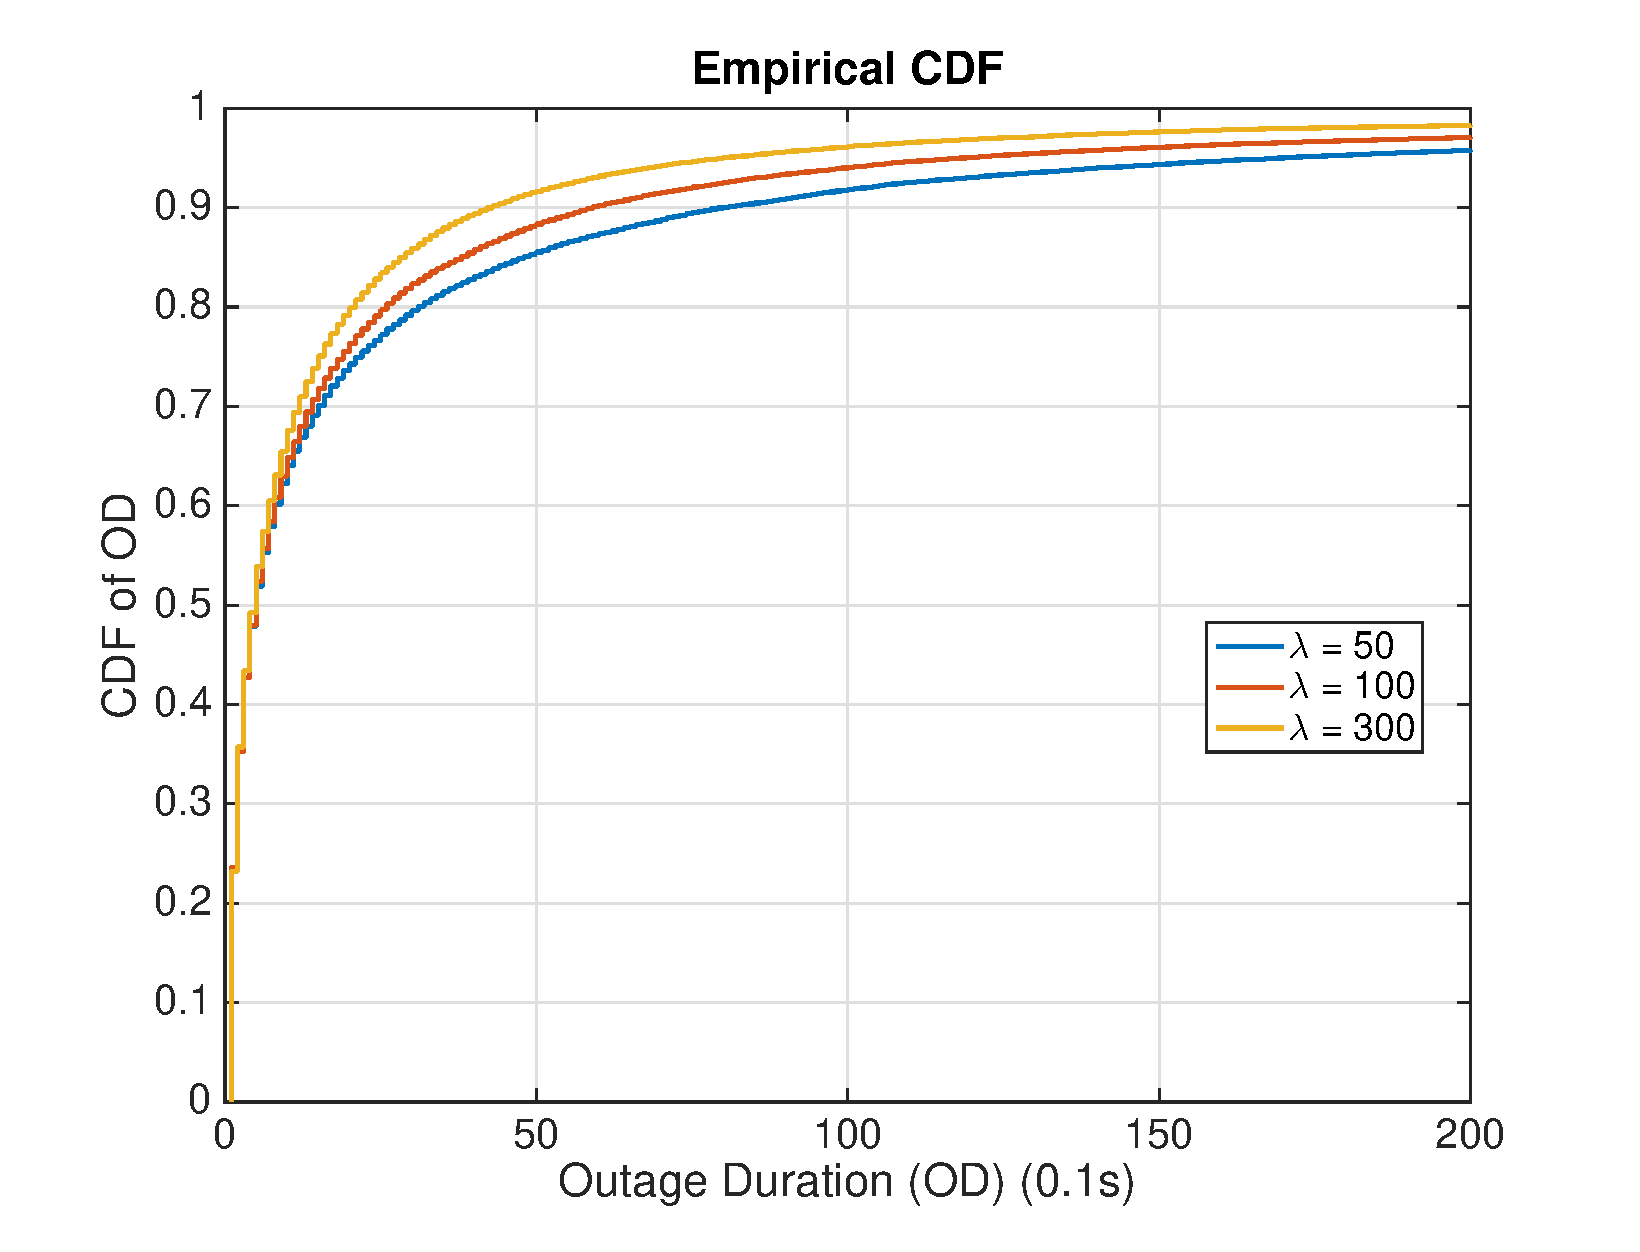
\includegraphics[width=10cm]{ODthresh-5DeCorr200NBMode2.eps}
 \caption{CDF of Outage Durations when MS is connecting to the Nearest BS with correlated shadowing (de-correlation distance: 200m)}
 \label{corr1}
 \end{figure}
 \begin{figure}
 \centering
 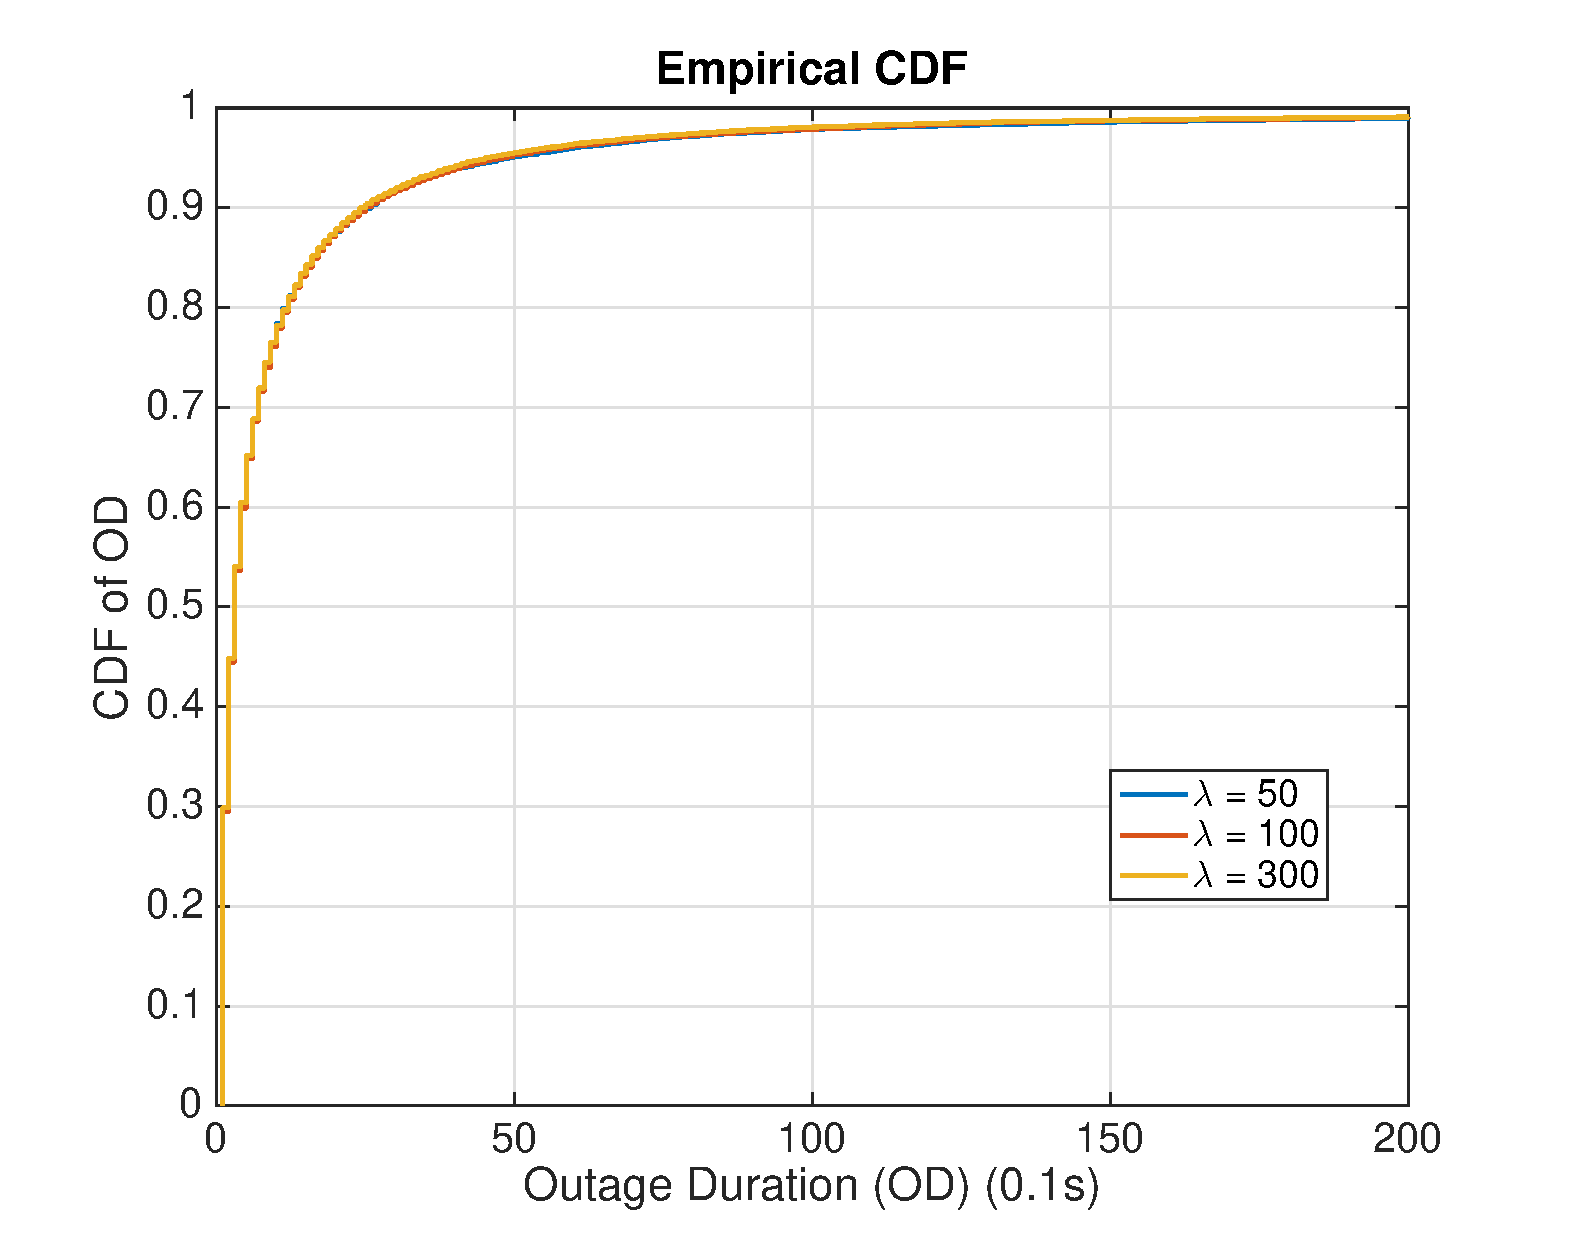
\includegraphics[width=10cm]{ODthresh-5DeCorr200MaxMode2.eps}
 \caption{CDF of Outage Durations when MS is connecting to the Strongest BS with correlated shadowing (de-correlation distance: 200m)}
 \label{corr2}
 \end{figure}
 \par Next, we move forward to investigate the system performance when the MS chooses to connect to the BS, which provides the highest SINR. The same simulations as the nearest BS scenario are executed to explore this scenario. Figure \ref{4:Mode12}, \ref{4:Mode22} and \ref{4:Mode32} present the receiving SINR of the MS when connecting to the strongest BS. In Figure \ref{4:Mode12}, \ref{4:Mode22} and \ref{4:Mode32}, CDF curves of SINR almost overlap each other when increasing BS densities, which means increasing BS density will not change the CDF of SINR significantly. Figure \ref{fig: outprobs2} shows the outage probability bars, which are consistent with our conclusion. For each shadow fading model, the difference between the highest outage probability and the lowest outage probability is less than $5\%$. Comparing three different shadow fading models, we can conclude that when the MS is connecting to the strongest BS, long de-correlation distance will harm the system performance by increasing the outage probability (yellow bars are higher than green or blue bars). 
 \par Comparing Figure \ref{fig: outprob1} with Figure \ref{fig: outprobs2}, we find that with the same BS density, outage probabilities are lower for every shadow fading model if MS is connecting to the strongest BS. For example, with the independent shadow fading and the BS density being $50$, the outage probability of the Nearest BS mode is $38\%$, while this probability of the Strongest BS mode is $6\%$. For correlated shadow fading with the de-correlation distance being $200m$ and the BS density being $50$, we find that the outage probability of the Nearest BS mode is around $30\%$. This is higher than that of the Strongest BS mode, which is $14\%$. Therefore, we conclude that connecting to the BS which provides highest SINR will improve the system performance with regard to the same network setup. 








 \par In the end, we investigate the system performance from the perspective of outage duration. We use the Random Waypoint mobility model to model the user mobility. The parameters of the Random WayPoint model are given in Table \ref{RWP}. The MS speed is assumed to be between $1m/s$ (pedestrian speed) and $20m/s$ (highway car speed). The MS pause interval is assumed to be uniformly distributed between $0s$ to $60s$. The simulation time is set to be $0.1s$, which means we check the MS's SINR every $0.1s$ to determine if it is in the outage area or not. Simulation results are shown in Figure \ref{iid1}, \ref{corr1}, \ref{iid2} and \ref{corr2}. Comparing Figure \ref{iid1} and Figure \ref{corr1}, Figure \ref{iid2} and Figure \ref{corr2}, we conclude that when the channel is under independent shadow fading, the outage duration is usually less than $2s$. However,  when the channel is under correlated shadow fading with $200m$ de-correlation distance, the outage duration can be longer than $20s$. Therefore, we draw the conclusion that correlated shadow fading leads to long-lasting outage durations and deteriorate the system performance. Comparing Figure \ref{iid1} and Figure \ref{iid2}, we find that connecting to the strongest BS will reduce the outage duration. For example, the percentage of outage durations of the Nearest BS mode with a length less than $0.5s$ is $94\%$, while that of the Strongest BS mode is $100\%$.  Figure \ref{corr1} and Figure \ref{corr2} confirm this conclusion in addition. For example, the percentage of outage durations less than $5s$ in Figure \ref{corr1} is $85\%$ with BS density being $50$. However, this percentage in Figure \ref{corr2} is increased to $95\%$. Furthermore, Figure \ref{corr1} indicates that increasing the BS density will reduce the percentage of long-lasting outage durations if the MS is connecting to the nearest BS. For example, in Figure \ref{corr1}, when the BS density increases from $50$ to $300$, the percentage of outage durations longer than $5s$ is reduced from $15\%$ to $8\%$. In contrast, for independent shadow fading and correlated shadow fading with the MS connecting to the strongest BS, increase the BS density will not change the distribution of outage durations, which is confirmed by Figure \ref{iid1}, Figure \ref{iid2} and Figure \ref{corr2}. All CDF curves of outage durations are the same with different BS densities. 
 \begin{table}
 \centering
 \caption{\label{RWP}Random Waypoint Mobility Model Parameters}

 \begin{tabular}{|c|c|}

 \hline
 Speed Interval & $1m/s - 20m/s$\\
 \hline
 Pause Interval & $0s - 60s$\\
 \hline
 Sample Time & $0.1s$\\
 \hline
 \end{tabular}

 \end{table}

 \section{Chapter Summary}
 \label{4:Conclusion}
 Shadow fading is a large-scale fading, which can cause significant received power loss for a wide area. In general, shadow fading is considered to be independent log-normal distributed to simplify the analysis; however, this is not the real case. In reality, shadow fading at two different positions are correlated to each other. Correlated shadow fading will result in correlated outage events and long-lasting outage durations. To investigate the performance of a multi-cell system given correlated shadow fading, simulations are implemented to analyze the outage probability and the outage duration distribution. First of all, the probability of two different BS layouts: Grid model and Random model are investigated. We find that the Grid model performs better than the Random model. Secondly, outage probabilities given different BS densities and two different connecting strategies: Nearest BS mode and Strongest BS mode, are simulated. We conclude that connecting to the strongest BS will reduce the outage probability compared with the nearest BS from simulation results. Increasing the BS density will not reduce the outage probability when the MS is connecting to the strongest BS. However, when the MS is connecting to the nearest BS and the de-correlation distance of correlated shadow fading is large enough, increasing the BS density will reduce the outage probability.  Finally, we analyze the system performance in terms of outage duration. Simulation results show that correlated shadow fading will result in long-lasting outage durations. Simulation results show that increasing the BS density will reduce the percentage of long-lasting outage durations if the MS chooses to connect to the nearest BS. Therefore, we suggest dense BS layout might be a proper strategy for next generation mmWave communication networks with correlated shadow fading.
 

